\documentclass[a4paper, 11pt, ngerman, parskip=half-]{scrartcl}

\title{MoF -- Fragenkatalog}
\subtitle{\href{https://github.com/Bierbunker/MoF-Ausarbeitung}{\underline{Aktuelle Version (Link)}}}
\date{\today}

\usepackage[margin=1in]{geometry}

\usepackage[utf8]{inputenc}
\usepackage[T1]{fontenc}
\usepackage{lmodern}
\usepackage{babel}
\usepackage{csquotes}
\usepackage{xurl}

\usepackage{amsmath, amssymb, amstext, mathtools}
\usepackage{icomma}
\usepackage[locale=DE, uncertainty-mode=separate]{siunitx}
\usepackage{physics}
\usepackage{derivative}  % overrides derivatives of package physics!

\usepackage{pdfpages}
\usepackage{lastpage}
\usepackage{graphicx}
\usepackage{float}
\usepackage{mhchem}
\usepackage{chemformula}
\usepackage{xcolor}
\usepackage[hidelinks,colorlinks]{hyperref}
%Colorlinks setup:
\hypersetup{
    colorlinks = false,
    linkbordercolor = {white}
}

\usepackage[headsepline]{scrlayer-scrpage}
\pagestyle{scrheadings}
\setkomafont{pageheadfoot}{\normalfont}
\ihead{\hyperlink{Fehler}{\color{cyan}Fehlermeldungen}}
\chead{MoF Fragenkatalog}
\ohead{\today}
\cfoot{\pagemark{} / \pageref*{LastPage}}

\usepackage{caption, subcaption}
\captionsetup[table]{name=Tabelle}
\captionsetup[figure]{name=Abbildung}
\captionsetup{format=plain, font=small, labelfont=bf, justification=centering}

% Line break after paragraph
\newcommand{\myparagraph}[1]{\paragraph{#1}\mbox{}\\}

% numerical aperture
\newcommand{\NA}{\ensuremath{\mathit{NA}}}


% Question command
\newcounter{question}
\newcommand{\question}[1]{\stepcounter{question}\paragraph{Frage \thequestion: #1}~}

\newcommand{\qref}[1]{%
  \phantomsection\label{q:#1}% Create a label for the question
  \textbf{\hyperref[q:#1]{#1}}% Link to the question label
}

\newcommand{\aqref}[1]{%
  \phantomsection\label{q:#1}% Create a label for the question
  \textbf{\hyperref[q:#1]{Frage #1}}% Link to the question label
}

\begin{document}

\maketitle

\newpage

\tableofcontents
\newpage
\section{Notizen aus der Vorlesung}
Magnetismus wird wahrscheinlich nicht zur Prüfung am 26. kommen. (Cat 15.06.)

Surnev will \textbf{viel Mathematik} und \textbf{wenig Text} bei der VO-Prüfung sehen. (Jax 21.06.)
\newpage
\section*{Ähnliche Fragen vermutlich (GPT-4)}

Einige Fragen sind ähnlich oder decken ähnliche Themen ab. Hier sind die entsprechenden Paare:

Fragen \qref{1} und \qref{13} diskutieren die Austauschenergie beim H2 Molekül und ihre Bedeutung für die chemische Bindung.

Fragen \qref{2} und \qref{14}, \qref{21}, \qref{32}, \qref{40} und \qref{55} fragen nach Informationen, die aus dem Rotations-Schwingungsspektrum von Molekülen abgeleitet werden können.

Fragen \qref{3} und \qref{15} behandeln elektrische Rotations-Schwingungsübergänge und die Entstehung von Schwingungsbanden.

Fragen \qref{4} und \qref{16}, \qref{27} und \qref{45}, \qref{50} und \qref{54} beziehen sich auf den Zusammenhang zwischen der Gitterebene und einem Vektor im reziproken Raum.

Fragen \qref{5} und \qref{17}, \qref{47} und \qref{59} beziehen sich auf das Auftreten von Energiebandlücken mit Hilfe des Models der fast freien Elektronen.

Fragen \qref{6} und \qref{18} behandeln, wie experimentell die Dispersionsrelationskurve von Phononen ermittelt werden kann.

Fragen \qref{7} und \qref{19}, \qref{38}, \qref{51} und \qref{57} diskutieren die Wärmekapazität sowohl in der klassischen als auch in der quantenmechanischen Betrachtung.

Fragen \qref{8} und \qref{20} beziehen sich auf das Bloch-Theorem eines Elektrons im harmonischen Potential.

Fragen \qref{9} und \qref{56} behandeln den Paulschen Paramagnetismus.

Fragen \qref{24} und \qref{37} beziehen sich auf die Hybridisierung in mehratomigen Molekülen.

Fragen \qref{25} und \qref{35}, \qref{44} behandeln die Laue'sche Beugungsbedingung und die Ewald-Konstruktion.

Fragen \qref{26} und \qref{36} diskutieren den Unterschied zwischen einem fcc-Gitter und einer hcp-Struktur.

Fragen \qref{28} und \qref{39}, \qref{48} und \qref{58} vergleichen die Einstein- und Debye-Modelle der spezifischen Wärme.

Fragen \qref{30} und \qref{49} erläutern den Atomfaktor und den Strukturfaktor bei der Röntgenbeugung.

Fragen \qref{41} und \qref{52} behandeln die Lennard-Jones-Potential und Van der Waals Bindung.

Fragen \qref{42} und \qref{33} behandeln das Konzept des Bravaisgitters und der Wigner-Seitz Zelle.

Fragen \qref{43} und \qref{31}, \qref{34} diskutieren das Franck-Condon Prinzip und die Intensität von Schwingungsbänden in einem Molekülspektrum.

Es ist wichtig zu beachten, dass obwohl diese Fragen ähnliche Themen behandeln, die spezifischen Aspekte oder der Kontext, der in jeder Frage behandelt wird, variieren können. Daher ist es wichtig, jede Frage sorgfältig zu lesen und zu verstehen, bevor man versucht, sie zu beantworten.

\newpage
\section{01. Mai 2015}
\question{Austauschenergie beim H2 Molekül? Wann ist es groß/klein? Wieso ist es für die Bindung wichtig?}
\label{q:1}

Die Austauschenergie oder oft auch \textbf{Austauschwechselwirkung} spielt bei der chemischen Bindung eine bedeutende Rolle. \\
Sie ist groß, falls sich die Atomorbitale stark überlappen---sprich symmetrisch sind---und kleiner falls sie sich weniger überlappen (=anti-symmetrisch). \\
Wie man in der Abbildung erkennen kann, ergibt sich eine Bindung nur, wenn die Orbitale sich überlappen (im symmetrischen Fall $U_S$). \\
\begin{figure}[H]  
    \centering
    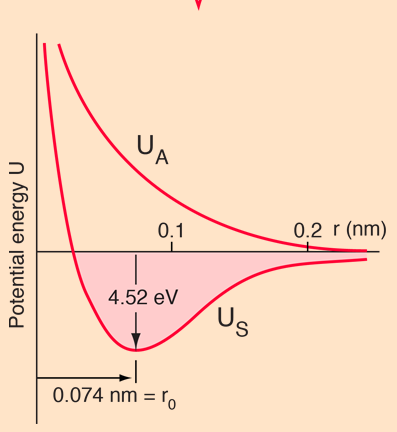
\includegraphics[width=.4\textwidth]{resources/05-01-2015/Frage1.png}
    \caption{siehe \href{http://hyperphysics.phy-astr.gsu.edu/hbase/molecule/hmol.html}{LINK}}
\end{figure}

\question{Was kann man aus dem Rotations-Schwingungsspektrum für molekulare Größen bestimmen?}
\label{q:2}

Unter Annahme, dass die beiden Atome ihren Abstand bei Rotation nicht ändern kann man den \textbf{Bindungsabstand} $R_e$ bestimmen. \\
Weiter lässt sich die \textbf{Rotationskonstante} $B_e$ bzw. deren anharmonischer Anteil $\alpha_e$, die \textbf{Schwingungsfrequenz} $\omega$ und das \textbf{Trägheitsmoment} $I$ bestimmen. \\

\[B_e = \frac{\hbar}{4 \pi c M R_e^2}\text{\quad [cm$^{-1}$]}\]
\[E_{rot} = \frac{\hbar^2}{2 I} \cdot J(J+1)\text{\quad [J]}\]
\[E_{rot} = B_e \cdot h\cdot c\]
$J$ ist dabei die Quantenzahl der Rotation und $M$ die reduzierte Masse (damit $M * R_e^2$ eben $I$ entspricht; gilt freilich nur für 2-Atom Systeme). \\

\[\Delta E_{rot} = \frac{(J+1)\hbar^2}{M\cdot {R_e}^2}\]
\[\Delta E_{vib} = \hbar \cdot \omega\]

\question{Diskutieren Sie elektrische Rotations-Schwingungsübergänge und die Entstehung von Schwingungsbanden.}
\label{q:3}

Übergänge zwischen Schwingungs-Rotations-Niveaus ($f_i$,$J_i$) $\rightarrow$ ($f_j$,$J_j$) innerhaltb desselben elektronischen Zustandes bilden für $f_i \neq f_j$ ein Schwingungs-Rotations-Spektrum. \\

\textbf{WICHTIG:} nur Moleküle welche ein permanentes Dipolmoment besitzen können solche Übergänge durchführen (z.B.: \ce{CO2}, \ce{H2O} aber \underline{nicht} \ce{O2}, andere homonuklearen, \dots etc.). \\

Wird Energie (Photon) von außen zugeführt oder abgegeben, so kann ein Übergang zwischen den Niveaus stattfinden - Auswahlregel $\Delta J = \pm 1$. Sprich Rotations-Schwingungsübergänge spielen sich zwischen benachbarten Niveaus ab.\\

\textbf{Schwingungsbanden} bezeichnen nun alle Rotationslinien welche zu einem Schwingungsübergang gehören. \\


\question{Was für ein Zusammenhang besteht zwischen der Gitterebene und einem Vektor im reziproken Raum?}
\label{q:4}

Der Abstand zweier Gitterebenen $d_{hkl}$ ist gegeben durch:
\[d_{hkl} = \frac{a}{\sqrt{h^2 + k^2 + l^2}}\]
und hängt mit dem reziproken Gittervektor $\vec{G_{hkl}}$ 
\[\vec{G_{hkl}} = h\vec{b_1} + k\vec{b_2} + l\vec{b_3}\]
wie folgt zusammen:
\[d_{hkl} = \frac{2\pi}{|\vec{G_{hkl}}|}\]

Somit ist die Länge des reziproken Gittervektors $\vec{G_{hkl}}$ indirekt proportional zum Abstand der Gitterebenen $d_{hkl}$.

\question{Erklären Sie das Auftreten von Energiebandlücken mit Hilfe des Models der fast freien Elektronen.}
\label{q:5}

Als Bandlücke, wird der energetische Abstand zwischen Valenzband und Leitungsband eines Festkörpers bezeichnet. Dessen elektrische und optische Eigenschaften werden wesentlich durch die Größe der Bandlücke bestimmt.
Nach dem Bändermodell sind gebundene Zustände der Elektronen nur auf bestimmten Intervallen der Energieskala zugelassen, den Bändern. Zwischen den Bändern können energetisch verbotene Bereiche liegen. Jeder dieser Bereiche stellt eine Lücke zwischen den Bändern dar, jedoch ist für die physikalischen Eigenschaften eines Festkörpers nur die eventuelle Lücke zwischen dem höchsten noch vollständig mit Elektronen besetzten Band und dem nächsthöheren von entscheidender Bedeutung. Daher ist mit der Bandlücke immer diejenige zwischen Valenz- und Leitungsband gemeint.
Das Auftreten einer solchen lücke lässt sich durch das Modell der quasifreien Elektronen beschreiben. Dabei wird das Modell freier Elektronen, welches das erhalten der Valenzelektronen in einer kristallinen Struktur eines festen Metalls darstellt, durch ein elektrostatisches periodisches Potential
erweitert. Dadurch kommt es zu einer näherungsweisen Beschreibung der positive geladenen Atomrümpfe im Kristallgitter. Man setzt dabei zunächst die Periodizität der Energiebänder im reziproken Raum an, welche bei Berücksichtigung eines kleinen Gitterpotentials an den Zonengrenzen eine Bandlücke aufweisen. 
Diese Methode erlaubt eine theoretische Vorhersage der Bandlücke und damit eine Einteilung der Festkörper in elektrische Leiter, Halbleiter und Isolatoren.
Hierbei gilt als Faustregel:

\begin{itemize}
    \item Leiter: keine Bandlücke.
    \item Halbleiter: Bandlücke im Bereich von 0,1 bis ca. 3 eV.
    \item Nichtleiter: Bandlücke größer als 3 eV.
\end{itemize}

\question{Wie kann experimentell die Dispersionsrelationskurve von Phononen ermittelt werden?}
\label{q:6}

\begin{figure}[H]  
    \centering
    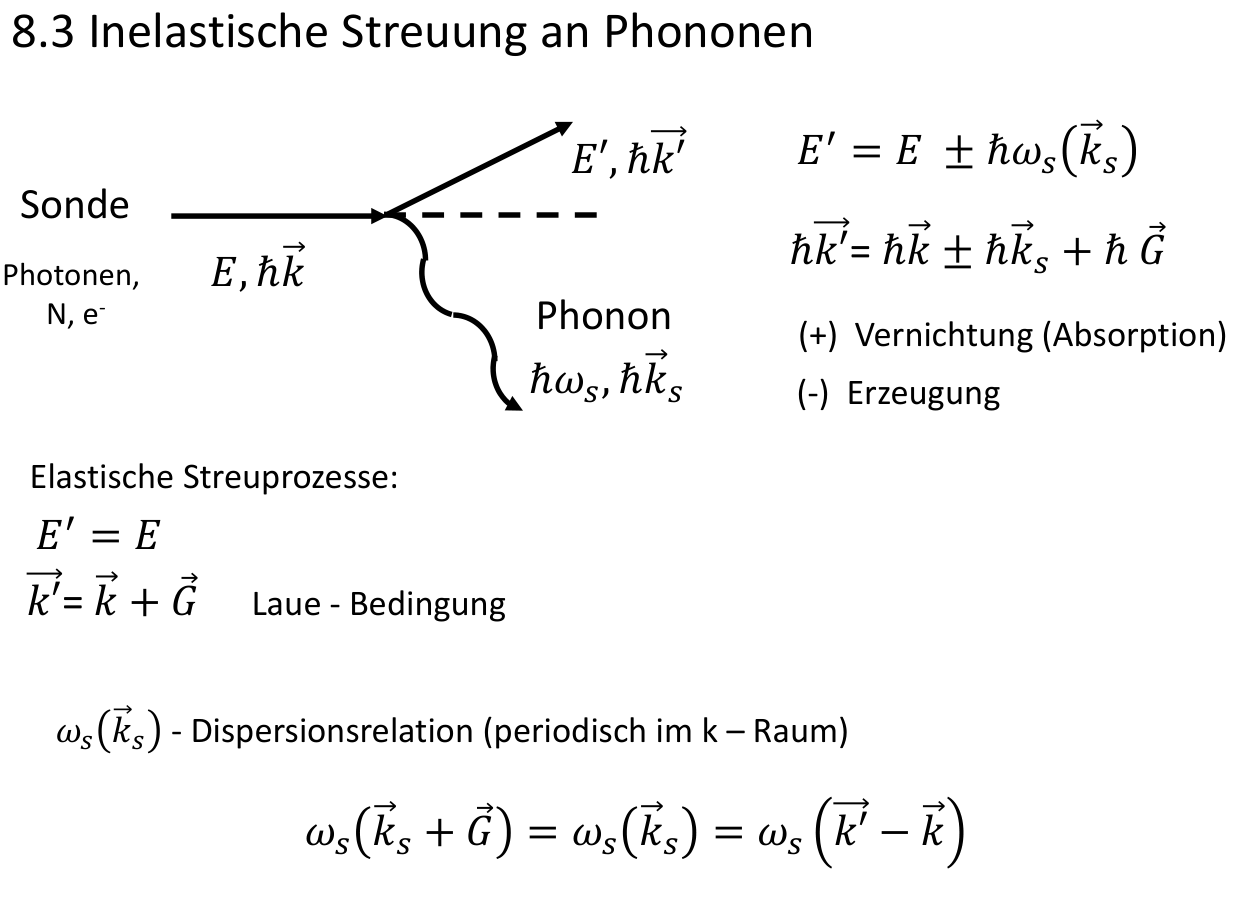
\includegraphics[width=.8\textwidth]{resources/05-01-2015/Frage6_1.png}
    \caption{Inelastische Streuung an Phononen}
\end{figure}

\begin{figure}[H]  
    \centering
    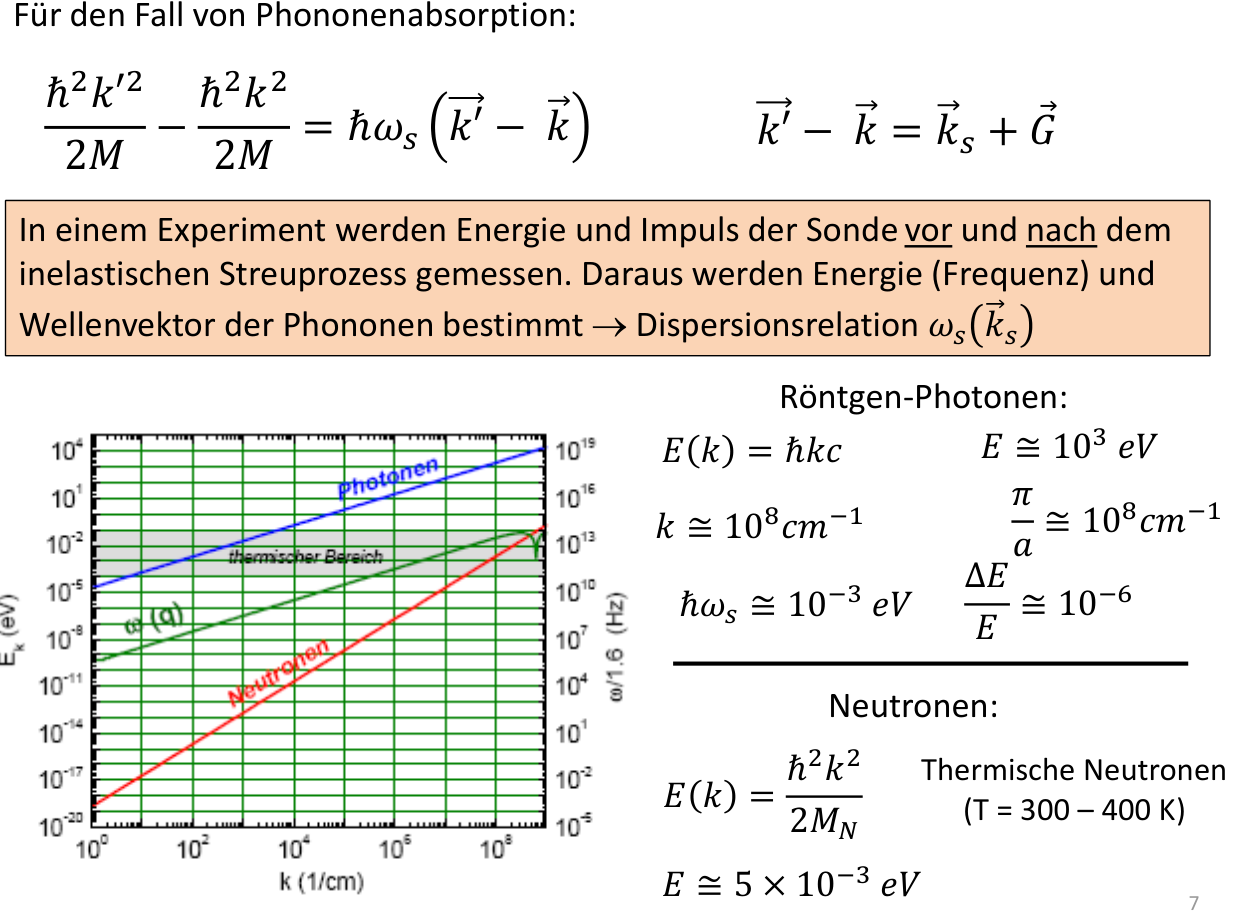
\includegraphics[width=.8\textwidth]{resources/05-01-2015/Frage6_2.png}
    \caption{Dispersionsrelation Phononen in einem Experiment}
\end{figure}

\question{Diskutieren Sie die Wärmekapazität sowohl in der klassischen als auch in der quantenmechanischen Betrachtung.}
\label{q:7}

In der der klassischen Physik wird angenommen, dass die Energieauf- und abnahme eines Materials 
kontinuerlich ist bzw. die Energieniveaus von Molekülen und Atomen eines Materials kontinuierlich 
variieren können. \\
In den quantenmechanischen Modellen können die Energieniveaus nur diskrete Werte annehmen, wodurch die 
Wärmekapazität eines Materials bei niedrigen Temperaturen diskrete Schritte 
aufweist, die durch die Energieniveaus der quantenmechanischen Zustände bestimmt sind (Einstein, Debye).
(Die Quantisierung der Gitterschwingungen ist entscheidend für die innere Energie und
die spezifische Wärme des Kristallgitters.)
\\
Bei hohen Temperaturen nähert sich die klassische Wärmekapazität der quantenmechanischen Wärmekapazität 
an (Abstände zwischen Energieniveaus wird kleiner).

\begin{figure}[H]  
    \centering
    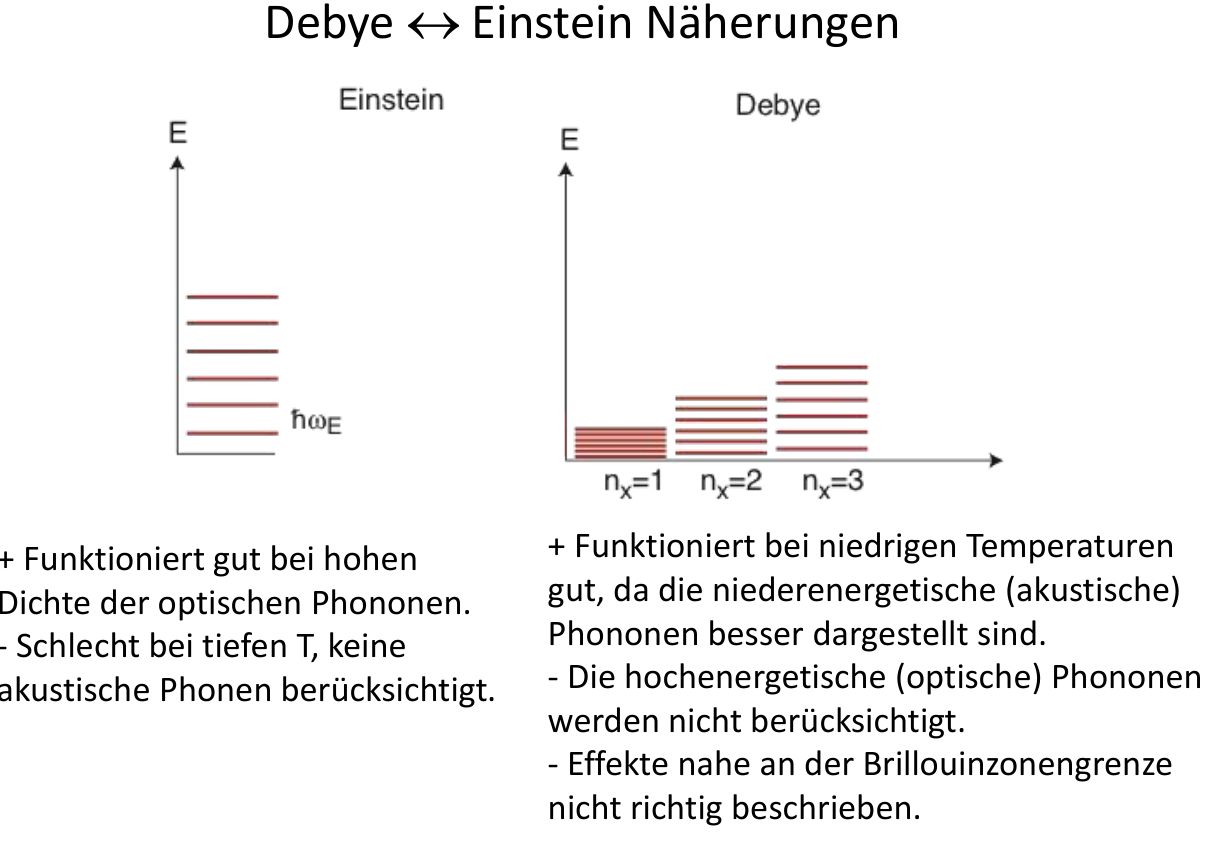
\includegraphics[width=.8\textwidth]{resources/05-01-2015/Frage7.png}
    \caption{Vergleich zwischen Einstein- und Debye-Modell.}
\end{figure}

\question{Beschreiben Sie das Bloch-Theorem eines Elektrons im harmonischen Potential.}
\label{q:8}
Das Bloch-Theorem beschreibt das Verhalten eines Elektrons in einem periodischen Potential. Dabei nimmt das Elektron eine spezielle Wellenfunktion an, die als Bloch-Funktion bezeichnet wird. Diese Bloch-Funktion hat die Form einer ebene Welle, multipliziert mit einer periodischen Funktion, die die Symmetrie des Potentials widerspiegelt. \\

Im Fall eines harmonischen Potentials ergibt sich die Schrödinger-Gleichung für ein Elektron zu:
\begin{align}
 ((- \frac{\hbar^2}{2m }) \nabla ^2  + V(x)) \Psi (x) = E \Psi (x)
\end{align}

Hierbei ist $\hbar$ das reduzierte Planck'sche Wirkungsquantum, $m$ die Masse des Elektrons, $\nabla$ der Laplace-Operator, $\Psi (x)$ die Wellenfunktion des Elektrons, $V(x)$ das harmonische Potential und $E$ die Energie des Elektrons.
Für das Potential $V(\vec{r})$ gilt die \textbf{Translations-Invarianz}:
\begin{align}
    V(\vec{r}) = V(\vec{r} + \vec{R})
\end{align}
mit einem beliebigen Translationsvektor $\vec{R}$ im dreidimensionalen periodischen Gitter, welche aus einem Vielfachen der Basisvektoren besteht. \\

Allgemein ist das Potential $V(\vec{r})$ gitterperiodisch und lässt sich als Sume von harmonischen Funktionen in Abhängigkeit des Gittervektors $\vec{G}$ schreiben:

\begin{align}
    V(\vec{r}) = \sum_{\vec{G}} V_{\vec{G}} e^{i \vec{G} \vec{r}} \hspace{1cm} \mbox{mit} \hspace{1cm} V_{-G} = V_G*
\end{align}

Für die Lösung der Schrödingergleichung ist der Ansatz:
\begin{align}
    \Psi(\vec{r}) = \sum_{\vec{G}}  C_{\vec{k}} e^{i \vec{k} \vec{r}}
\end{align}
Der Ansatz erfüllt die periodischen Randbedingungen, wobei $\vec{k}$ ein Punkt im reziproken Raum ist. \\

Die Lösungen dieser Gleichung sind \textbf{Bloch-Funktionen}, die gegeben sind durch:
\begin{align}
    \Psi (\vec{r})) = \exp{(ik\vec{r})} u(\vec{r})
\end{align}

Hierbei ist k der Wellenvektor des Elektrons und $u(\vec{r})$ eine periodische Funktion mit derselben Periodizität wie das harmonische Potential. Die periodische Funktion $u(\vec{r})$ erfüllt die Gleichung:
\begin{align}
    u(\vec{r}) = u(\vec{r}+\vec{R})
\end{align}
wobei $\vec{R} $ der Gittervektor ist und so die Translations-Invarianz sowie die Periodizität des Potentials dargestellt wird. \\

Die Bloch-Funktionen sind ebenfalls symmetrisch bei Verschiebung um einen Vektor $\vec{G'}$:
\begin{align}
    \Psi _{\vec{k} + \vec{G'}} &= \Psi _{\vec{k}} (\vec{r}) \\
    E(\vec{k} + \vec{G'}) &= E(\vec{k})
\end{align}

Das Bloch-Theorem besagt, dass die Bloch-Funktionen eine vollständige Basis des Lösungsraums der Schrödinger-Gleichung im harmonischen Potential darstellen. Das bedeutet, dass jede Wellenfunktion $\Psi(x)$ eines Elektrons in diesem Potential als Linearkombination der Bloch-Funktionen dargestellt werden kann. \\


Das Bloch-Theorem ist von entscheidender Bedeutung für das Verständnis des elektronischen Verhaltens in Festkörpern, da es erklärt, warum Elektronen bestimmte \textbf{Energiebänder} bilden und sich diese Bänder wiederum in isolierende, leitende und halbleitende Eigenschaften des Materials manifestieren.

\begin{figure}
    \centering
    \includegraphics{xxx}
    \caption{Darstellung der Elektronischen Bandstruktur.}
\end{figure}

\question{Beschreiben Sie den Paulschen Paramagnetismus.}
\label{q:9}

\question{Potentiat-Bindung im homöopolaren Molekül?}
\label{q:10}
Siehe Frage \ref{q:11}


\newpage

\section{05. Mai 2015}

\question{Skizzieren Sie den Verlauf der Potentialkurve für ein homöopolares Molekül. Erklären Sie sie qualitativ.}
\label{q:11}

(Siehe auch \aqref{2}.)

Homöopolare Moleküle sind Moleküle, die aus Atomen desselben Elements bestehen. Sie entstehen durch kovalente Bindungen. In Abbildung \ref{fig:Frage_11} ist die Potentialkurve einer kovalenten Bindung dargestellt, welche mit einem Lennard-Jones-Potential angenähert werden kann. Für kleine Abstände dominiert der Faktor $\frac{a}{R^{12}}$ (Abstoßung der Elektronen durch Pauli-Prinzip) bei größeren Abständen der Faktor $-\frac{b}{R^6}$ (Van der Waals). Die Bindungsenergie $E_B = \frac{b^2}{4a}$ befindet sich beim globalen Minimum.

\textcolor{red}{\textbf{Caveat:}} In \autoref{fig:Frage_11} ist die Bindungsenergie $E_B = \frac{b^2}{4a}$ falsch berechnet, siehe etwa \href{https://en.wikipedia.org/wiki/Lennard-Jones_potential#Alternative_notations_of_the_Lennard-Jones_potential}{Wikipedia} oder selbst händisch nachrechnen!

\begin{figure}[H]
    \centering
    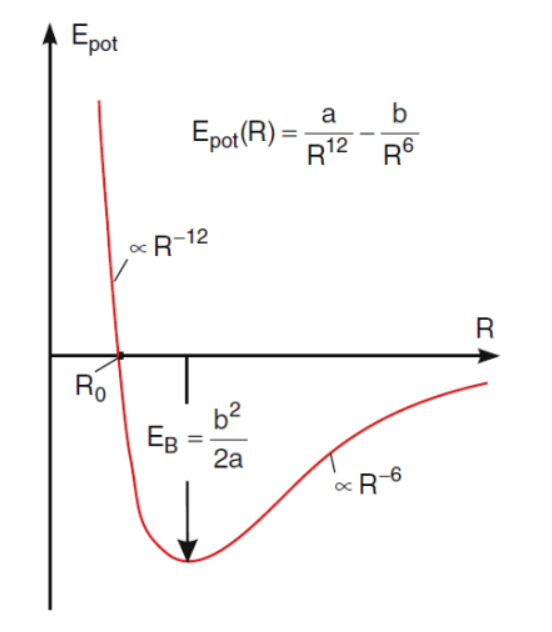
\includegraphics[width = 0.4\textwidth]{resources/05-05-2015/Frage_11.png}
    \caption{Potentialkurve homöopolare Molekül}
    \label{fig:Frage_11}
\end{figure}


\question{Erklären Sie die Herkunft der \enquote{Austauschenergie} in \ch{H2}. Wann ist sie groß, wann klein? Warum ist sie entscheidend für die chemische Bindung?}
\label{q:12}

Siehe \aqref{1}.

\question{Welche Informationen über molekulare Kenngrößen können aus Rotationsschwingungsspektren von Molekülen erhalten werden?}
\label{q:13}

(Siehe auch \aqref{2}.)

Es können folgende Kenngrößen bestimmt werden:
\begin{itemize}
    \item Gleichgewichtsabstand $R_e$
    \item Rotationskonstanten $B_e$ und $\alpha_e$
    \item Form der Potentialkurve
\end{itemize}

\question{Diskutiere einen elektronischen Übergang in einem 2-atomigen Molekül und die daraus resultierenden Schwingungsbanden im Spektrum.}
\label{q:14}

(Siehe auch \aqref{3}.)

Ändert sich die Schwingungsquantenzahl $\nu$, so ändert sich die Energie $E_{vib}$, bei Änderung der Rotationsquantenzahl $J$ die Energie $E_{rot}$. Die Gesamtenergie setzt sich aus der Schwingungs-, Rotations- und Potentialenergie zusammen:
\begin{equation}
    E = E_{rot} + E_{vib} + E_{pot}
\end{equation}
Der Abstand zwischen den einzelnen Energien $E_{rot}$ ist dabei deutlich kleiner als der zwischen den einzelnen Energien $E_{vib}$.\\
Übergänge zwischen Schwingungsrotationsniveaus $(\nu_i, J_i) \longleftrightarrow (\nu_k, J_k), \nu_i \neq \nu_k$: Schwingungsrotationsspektrum im infraroten Spektralbereich (\SIrange{2}{10}{\micro\meter})\\
Übergänge zwischen Schwingungsrotationsniveaus $(\nu_i, J_i) \longleftrightarrow (\nu_k, J_k), \nu_i = \nu_k$: Reines Rotationsspektrum, Mikrowellenbereich (\SIrange{e3}{e4}{\micro\meter})
\begin{figure}[H]
    \centering
    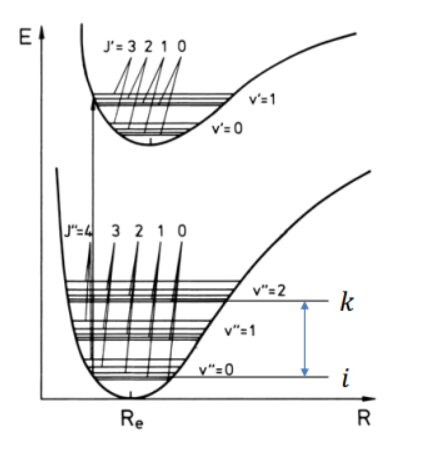
\includegraphics{resources/05-05-2015/Frage_14.png}
\caption{Übergänge zwischen Schwingungsrotationsniveaus}
    \label{fig:enter-label2}
\end{figure}

\question{Diskutiere den Zusammenhang zwischen Gitterebene im Kristall und Vektoren des reziproken Gitters.}
\label{q:15}

Siehe \aqref{4}.

\question{Diskutieren Sie die Wärmekapazität des Gitters im Rahmen des klassischen und der Quantenmechanik.}
\label{q:16}

(siehe auch \aqref{7}.)
%TODO: Bissl mehr Details

\textbf{Klassische Mechanik:}
\begin{itemize}
    \item Keine Translations- und Rotationsfreiheitsgrade
    \item Jedes Atom kann in 3 voneinander unabhängigen Raumrichtungen schwingen:
    \begin{itemize}
        \item 3 Schwingungsfreiheitsgrade der kinetischen Energie
        \item 3 Schwingungsfreiheitsgrade der potentiellen Energie
    \end{itemize}
\end{itemize}
Gesetz von Dulong-Petit:
\begin{equation}
    f = 6 \qquad c_\nu^m = 3N_Ak_B = 3R = \SI{24.9}{\joule\per\mole\per\kelvin}
\end{equation}

\textbf{Quantenmechanik}
Quantisierung der Gitterschwingungen entscheidend für die innere Energie und
die spezifische Wärme des Kristallgitters.\\
Bei niedrigen Temperaturen ($k_BT \ll \hbar\omega$) kommt es zu einem Ausfrieren der Schwingungsfreiheitsgrade:
\begin{equation}
    c_\nu^m \rightarrow 0
\end{equation}
Bei hohen Temperaturen ($k_BT \gg \hbar\omega$):
\begin{equation}
    c_\nu^m \rightarrow 3R \qquad \text{gleich wie beim Gesetzt von Dulong-Petit}
\end{equation}


\question{Wie ermittelt man experimentell eine Phononendispersionskurve?}
\label{q:17}

(siehe auch \aqref{6}.)

Durch Streuung von Photonen, Neutronen oder Elektronen am Kristallgitter. 

\begin{figure}[H]
    \centering
    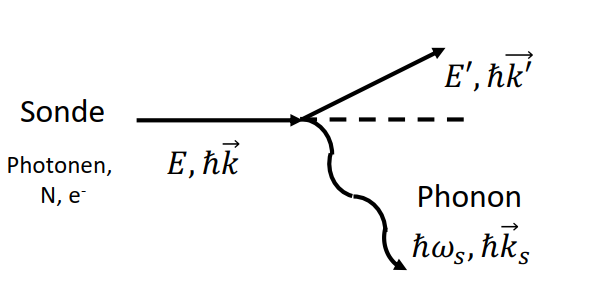
\includegraphics{resources/05-05-2015/Frage_17.png}
    \caption{Inelastische  Streuung an Phononen}
    \label{fig:enter-label}
\end{figure}
Die Dispersionsrelation ergibt sich dann zu:
\begin{equation}
    \omega_s(\vec{k_s})=\omega_s(\vec{k'}-\vec{k})
\end{equation}
Am besten durch Streuung von Neutronen: 
\begin{itemize}
    \item Energie und Impuls von Neutronen im selben Bereich wie Phononen
    \item Neutronen werden nur an Atomkernen gestreut und regen Gitterschwingungen an
\end{itemize}


\question{Erklären Sie das Zustandekommen von Energiebändern in Festkörper im Rahmen der Theorie der fast-freien Elektronen.}
\label{q:18}

Siehe \aqref{5}.

\question{Erklären Sie das Bloch'sche Theorem für Elektronen im periodischen Potential.}
\label{q:19}

Siehe \aqref{8}.

\question{Diskutieren Sie den Paulschen Paramagnetismus.}
\label{q:20}

\newpage

\section{09. Mai 2012}

\question{Skizzieren der wesentlichen Elemente der Born-Oppenheimer Näherung.}
\label{q:21}

Da die Atomkerne eine wesentlich größere Masse als die Elektronen haben und sich dadurch viel langsamer bewegen, ist es mit der Born-Oppenheimer
Näherung möglich die Positionen der Kerne zu fixieren. Somit lässt sich die molekulare Schrödingergleichung in eine für die Kerne und eine
für die Elektronen aufteilen.

\begin{itemize}
    \item Für die Elektronen stehen die Kerne still, wodurch ihre Lage als Parameter in das anziehende und abstoßende Potential eingeht.
        Somit hängen die elektronischen Eigenzustände und Energien nur von der Lage der Kerne ab und nicht von der Geschwindigkeit.\\
            Die Schrödingergleichung für die Elektronen lautet somit:
            
        \begin{align}
            \hat{H}_e \cdot \Phi_h(\vec{r},\vec{R}) = E_h(\vec{R}) \cdot \Phi_h(\vec{r},\vec{R})
        \end{align}

        Dabei ist $\vec{r}$ die Position der Elektronen und $\vec{R}$ die der Kerne. Der Hamilton-Operator besteht aus $\hat{H}_e = \hat{T}_e + \hat{V}_{ee} + \hat{V}_{eN}$, 
        also der kinetischen Energie der Elektronen + der Abstoßung zwischen den Elektronen + der Anziehung zwischen Kernen und Elektronen.

        \begin{equation}
            \label{eq:electronic_hamiltonian}
            H_{\text{elec}} = - \sum_i \frac{\hbar^2}{2m_e} \nabla^2_i - \sum_{a,i} \frac{Z_a e^2}{4 \pi \epsilon_0 |\vec{r}_i-\vec{r}_a| }  + \sum_{i<j} \frac{e^2}{4 \pi \epsilon_0 |\vec{r}_i-\vec{r}_j| }
        \end{equation}

    \item Die Kernbewegung ist von den Elektronen nahezu unbeeinflusst, jedoch bewegen sie sich im Potential der elektrischen Zustände. 
        Die Kern-Wellenfunktion $\eta_{hk}(\vec{R})$ hängt nur von der Kernkoordinate $\vec{R}$ ab.

        Die Schrödingergleichung lautet:
        \begin{align}
            (\hat{T}_n + \hat{V}_{NN} + E_h(\vec{R})) \cdot \eta_{hk}(\vec{R}) = E_{hk} \cdot \eta_{hk}(\vec{R})
        \end{align}
\end{itemize}



\question{Welche Informationen über molekulare Kerngrößen können aus Rotations-Schwingungsspektren von Molekülen erhalten werden?}
\label{q:22}

(siehe auch \aqref{2}.)

\begin{itemize}
    \item Rotationskonstanten $B_e$ und $\alpha_e$ 
    \item Gleichgewichtsabstand $R_e$
    \item Form der Potentialkurve
\end{itemize}
Die Rotationsenergieniveaus eines Moleküls sind direkt mit dessen Massenverteilung verbunden.
Die Kenntnis der Emissionslinien bzw. Absorbtionslinien (meistens $>\SI{800}{nm}$) ermöglicht es das Trägheitsmoment $I$ des Moleküls zu bestimmen.
\begin{align}
    E_{rot} &= \frac{J^2}{2I} \\
    E_{rot} &= \frac{\hbar^2}{2I}J(J+1) = BJ(J+1) \qquad J = 0,1,2 \qquad \text{QM} \\
    \Delta E_{rot} &= \frac{\hbar^2}{I}(J+1) = 2B(J+1)
\end{align}
Meist wird die Energie in der Spektroskopie in Form von Wellenzahlen (in \si{\per\meter}) angegeben, dies entspricht der räumlichen Frequenz der emittierten bzw. absorbierten E-Welle.
So kann ein Zusammenhang zur Rotationskonstante $B_e$ hergestellt werden.
\begin{align}
    F_{rot}(J) &= \frac{E_{rot}(J)}{h c} = B_e J(J+1) \\
    B_e &= \frac{\hbar}{4 \pi c I}
\end{align}

Die Schwingungsfrequenzen in einem Schwingungsrotationsspektrum geben Informationen über die Energieniveaus der Molekülschwingungen. 
Durch die Quantisierung der Schwingung kann man die Anzahl der Schwingungsmodi im Molekül bestimmen.
Die Schwingungsfrequenzen hängen von der Steifigkeit der Bindungen und der Masse der Atome ab.


\question{Diskutieren das Schwingungsrotationsspektrum eines 2-atomigen Moleküls.}
\label{q:23}

Siehe \aqref{43}.

\question{Welche Verbesserungen des einfachen MO- oder VB-Ansatzes ermöglichen eine bessere Übereinstimmung mit den experimentellen Werten?}
\label{q:24}

\textbf{Elektroneninteraktion}:

Ein Ansatz zur Verbesserung des MO- oder VB-Ansatzes besteht darin, die Elektronenkorrelation zu berücksichtigen. 
Der einfache Ansatz vernachlässigt die Wechselwirkungen zwischen Elektronen, was zu Fehlern bei der Berechnung der Bindungsenergien und der Geometrie führen kann. 
Die Elektronenkorrelation kann durch Methoden wie der Konfigurationswechselwirkung (CI) oder der Dichtefunktionaltheorie (DFT) berücksichtigt werden. 
Diese Methoden erlauben eine bessere Behandlung der Elektronenkorrelation und führen zu genaueren Ergebnissen.

\textbf{Relativistische Effekte}:

Ein weiterer Ansatz besteht darin, relativistische Effekte zu berücksichtigen. 
Insbesondere bei schweren Atomen wie den Übergangsmetallen sind relativistische Effekte wichtig, da sie die Elektronenstruktur und die Bindungsenergien beeinflussen können.

\question{Was versteht man unter dem Franck-Condon-Prinzip? Diskutiere die Intensität von Schwingungsbanden in einem Molekülspektrum bei einem elektronischen Übergang anhand des Franck-Condon-Prinzips.}
\label{q:25}

\paragraph{Variante 1}

Das Franck-Condon-Prinzip besagt: 
\begin{mdframed}[backgroundcolor=yellow!20] % Profi
    Bei Absorption bzw. Emission eines Photons erfolgt die Änderung der Elektronenanordnung in einem Molekül vorzugsweise \enquote{so rasch} (vertikal), dass sich dabei die Lage und die Geschwindigkeit der Kerne nicht ändert.
\end{mdframed}

Beruht auf dem Prinzip, dass Zeitskalen der Anregung $\nu_{el} \approx \SI{e15}{\hertz}$ zwei bis drei Größenordnungen schneller als Kernschwingungen $\nu_{N} \approx \SI{e13}{\hertz}$ sind. 

Die Intensität von Schwingungsbanden hängt ab vom Überlapp der Wellenfunktionen der beiden Zustände. Wie in \autoref{fig:q25} gezeigt, sind die wahrscheinlichsten Übergänge (blau und grün) jene, deren Maximum der Wellenfunktionen senkrecht übereinander liegen. Übergänge zu anderen Schwingungszuständen sind ebenfalls möglich, jedoch weniger wahrscheinlich. 

\paragraph{Variante 2}

Das Frank-Condon Prinzip besagt, dass elektronische Übergänge so schnell stattfinden (im Bereich von \SI{e-15}{s}), dass der Kernabstand sich effektiv nicht ändert.
Diese hohe Geschwindigkeit des elektronischen Übergangs gegenüber der Kernbewegung wird durch die geringe Masse der Elektronen ermöglicht (analog zur Born-Oppenheimer-Näherung).

Wenn ein Molekül nun von einem elektronischen Zustand in einen anderen übergeht, so ist dieser Übergang umso wahrscheinlicher, je mehr die Vibrationswellenfunktionen der beiden Zustände zueinander kompatibel sind (z. B. beim gleichen Kernabstand ein Maximum haben), siehe \autoref{fig:q25}.

Am Beispiel der Zustände in \autoref{fig:q25} bedeutet dies: Vom Vibrations-Grundzustand ($\nu'' = 0$) im elektronischen Grundzustand ist der wahrscheinlichste Übergang in den elektronisch angeregten Zustand derjenige, der im Vibrations-Zustand $\nu' = 2$ endet. Übergänge in andere Vibrations-Zustände können auch stattfinden, allerdings ist die Wahrscheinlichkeit dafür geringer.


\begin{figure}[H]
    \centering
    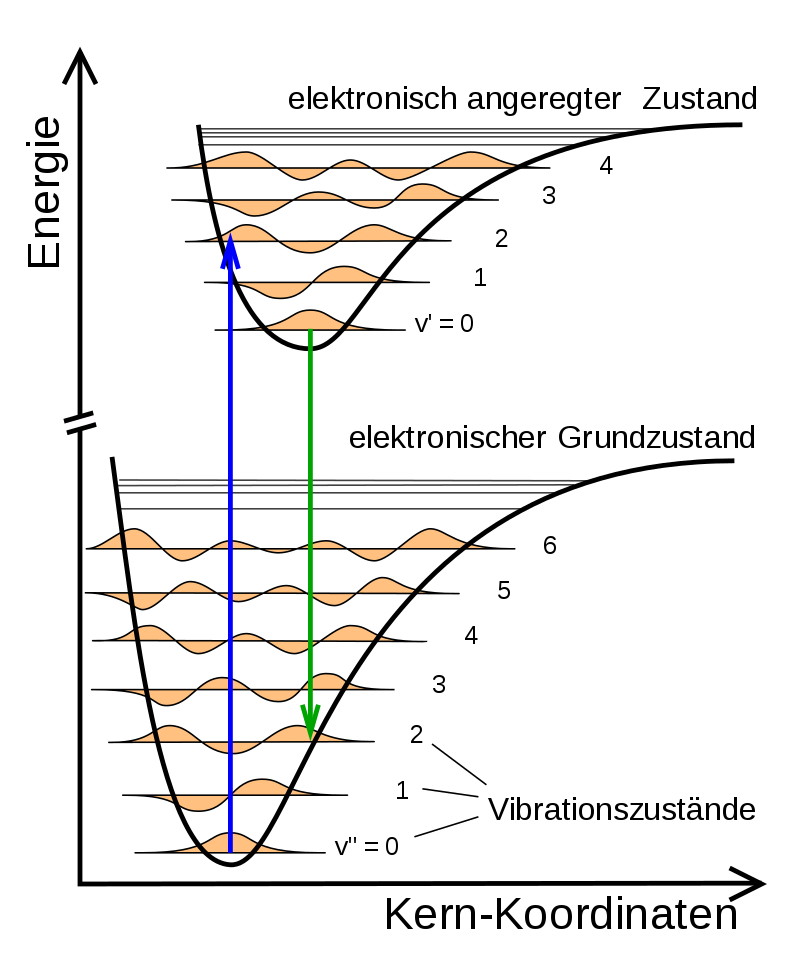
\includegraphics[width = 0.5\textwidth]{resources/09-05-2012/Franck-Condon-Prinzip}
    \caption{Schwarze Kurven: Energie eines zweiatomigen Moleküls in Abhängigkeit des Abstands der Kerne. Die Pfeile symbolisieren die vibronischen Übergänge.}
    \label{fig:q25}
\end{figure}


Um so einen Übergang zu modellieren, wird ein Dipoloperator eingeführt:
\begin{equation}
    \mu = \mu_{\epsilon} + \mu_K = - e \sum_{i} \vec{r_i}  + \sum_{j} Z_j \vec{R_j} 
\end{equation}
Die Übergangswahrscheinlichkeit zwischen den beiden Zuständen ist gegeben durch das Skalarprodukt
\begin{equation}
    P = \left\langle\psi| \mu | \psi' \right\rangle   
\end{equation}

während die Intensität $I$ des Übergangs das Quadrat dieser Übergangswahrscheinlichkeit ist: 
\begin{equation}
    I = |P|^2
\end{equation}
Die Wellenfunktionen der beiden Zustände (siehe \autoref{fig:q25}) können als Produkt der elektronischen und der Vibrationswellenfunktion ausgedrückt werden.
\begin{equation}
    \psi = \psi_{\epsilon}(\vec{r_i}) \psi_v(\vec{R_j})
\end{equation} 
Da der effektive Abstand der Kerne in den Zeitskalen des Übergangs sich nicht verändert kann angenommen werden, dass die Elektron-Positionen unabhängig von den Positionen der Kerne sind.
$\langle \psi_{\epsilon}' \psi_v' | \mu_{\epsilon}| \psi_{\epsilon} \psi_v\rangle  \approx  \langle\psi_v' |\psi_v \rangle \langle\psi_{\epsilon}'|\mu_{\epsilon}| \psi_{\epsilon} \rangle $ \\
Führt man nun das Skalarprodukt aus:
\begin{equation}
    P = \langle \psi_v' | \psi_v \rangle \langle \psi_{\epsilon}' | \mu_{\epsilon} | \psi_{\epsilon} \rangle + \langle \psi_{\epsilon}' | \psi_{\epsilon} \rangle \langle\psi_v' | \mu_K |\psi_v \rangle
\end{equation}
Die zwei elektronischen Wellenfunktionen sind orthogonal aufeinander und somit ist $\langle \psi_{\epsilon}' | \psi_{\epsilon} \rangle  = 0$.
Der erste Term quadriert $|\langle \psi_v' | \psi_v \rangle|^2$ ist der Frank-Condon-Faktor und der zweite Term das Übergangsdipolmoment. 
Die Intensität der Schwingungsbänder wird von der Überlappung der beiden Vibrationswellenfunktionen bestimmt.
\begin{equation}
    I = |\langle \psi_v' | \psi_v \rangle \langle \psi_{\epsilon}' | \mu_{\epsilon} | \psi_{\epsilon} \rangle|^2
\end{equation}


\question{Diskutiere die Laue'sche Beugungsbedingung: anhand Ewald Konstruktion im Rahmen der Bragg'schen Interpretation.}
\label{q:26}

\textbf{Bragg'sche Streubedingung:}
\begin{align}
    n\lambda = 2 d \sin{\Theta} 
\end{align}
\textbf{Von Laue Bedingungen:}
\begin{align}
\vec{G} &= \vec{k'} - \vec{k} \\
\vec{k} \cdot \vec{G} &= -\frac{1}{2} \vec{G}^2 \quad (*)
\end{align}
mit den Wellenvektoren $\vec{k}'$ (reflektierter Vektor) und $\vec{k}$ (einfallender Vektor), dem reziproken Gittervektor $\vec{G}$, sowie dem Ebenenabstand $d$ und dem Streuwinkel $\Theta$ Die Bragg-Bedingung ist ein Speziallfall der Laue-Bedingung. Es gelten folgende Relationen:
\begin{align}
    |\vec{G}_{hkl}| &= 2 |\vec{k}| \sin{\Theta} \\
    |\vec{k}| &= \frac{2 \pi}{\lambda} \\
    |\vec{G}_{hkl}| &= \frac{2 \pi n}{d_{hkl}}
\end{align}
und somit $n \lambda = 2 d_{hkl}  \sin{\Theta}$. \\
Konstruktive Interferenz findet immer statt, wenn der Wellenvektor des
einfallenden Strahls an der Grenze einer Brillouin Zone liegt. Die geometrische Darstellung mit der Ewald Konstruktion unter Berücksichtigung dieser Bedingungen ermöglicht es, den Beugungswinkel $\Theta$ und den Netzebenenabstand $d$ zu bestimmen. 

$(*)$ Herleitungsidee: man schreibt: $\vb{k}'-\vb{G} = \vb{k}$ quadriert auf beiden Seiten und setzt $k=k'$ (elastische Bedingung) ein. 

\begin{figure}[H]
    \centering
    \begin{samepage}
        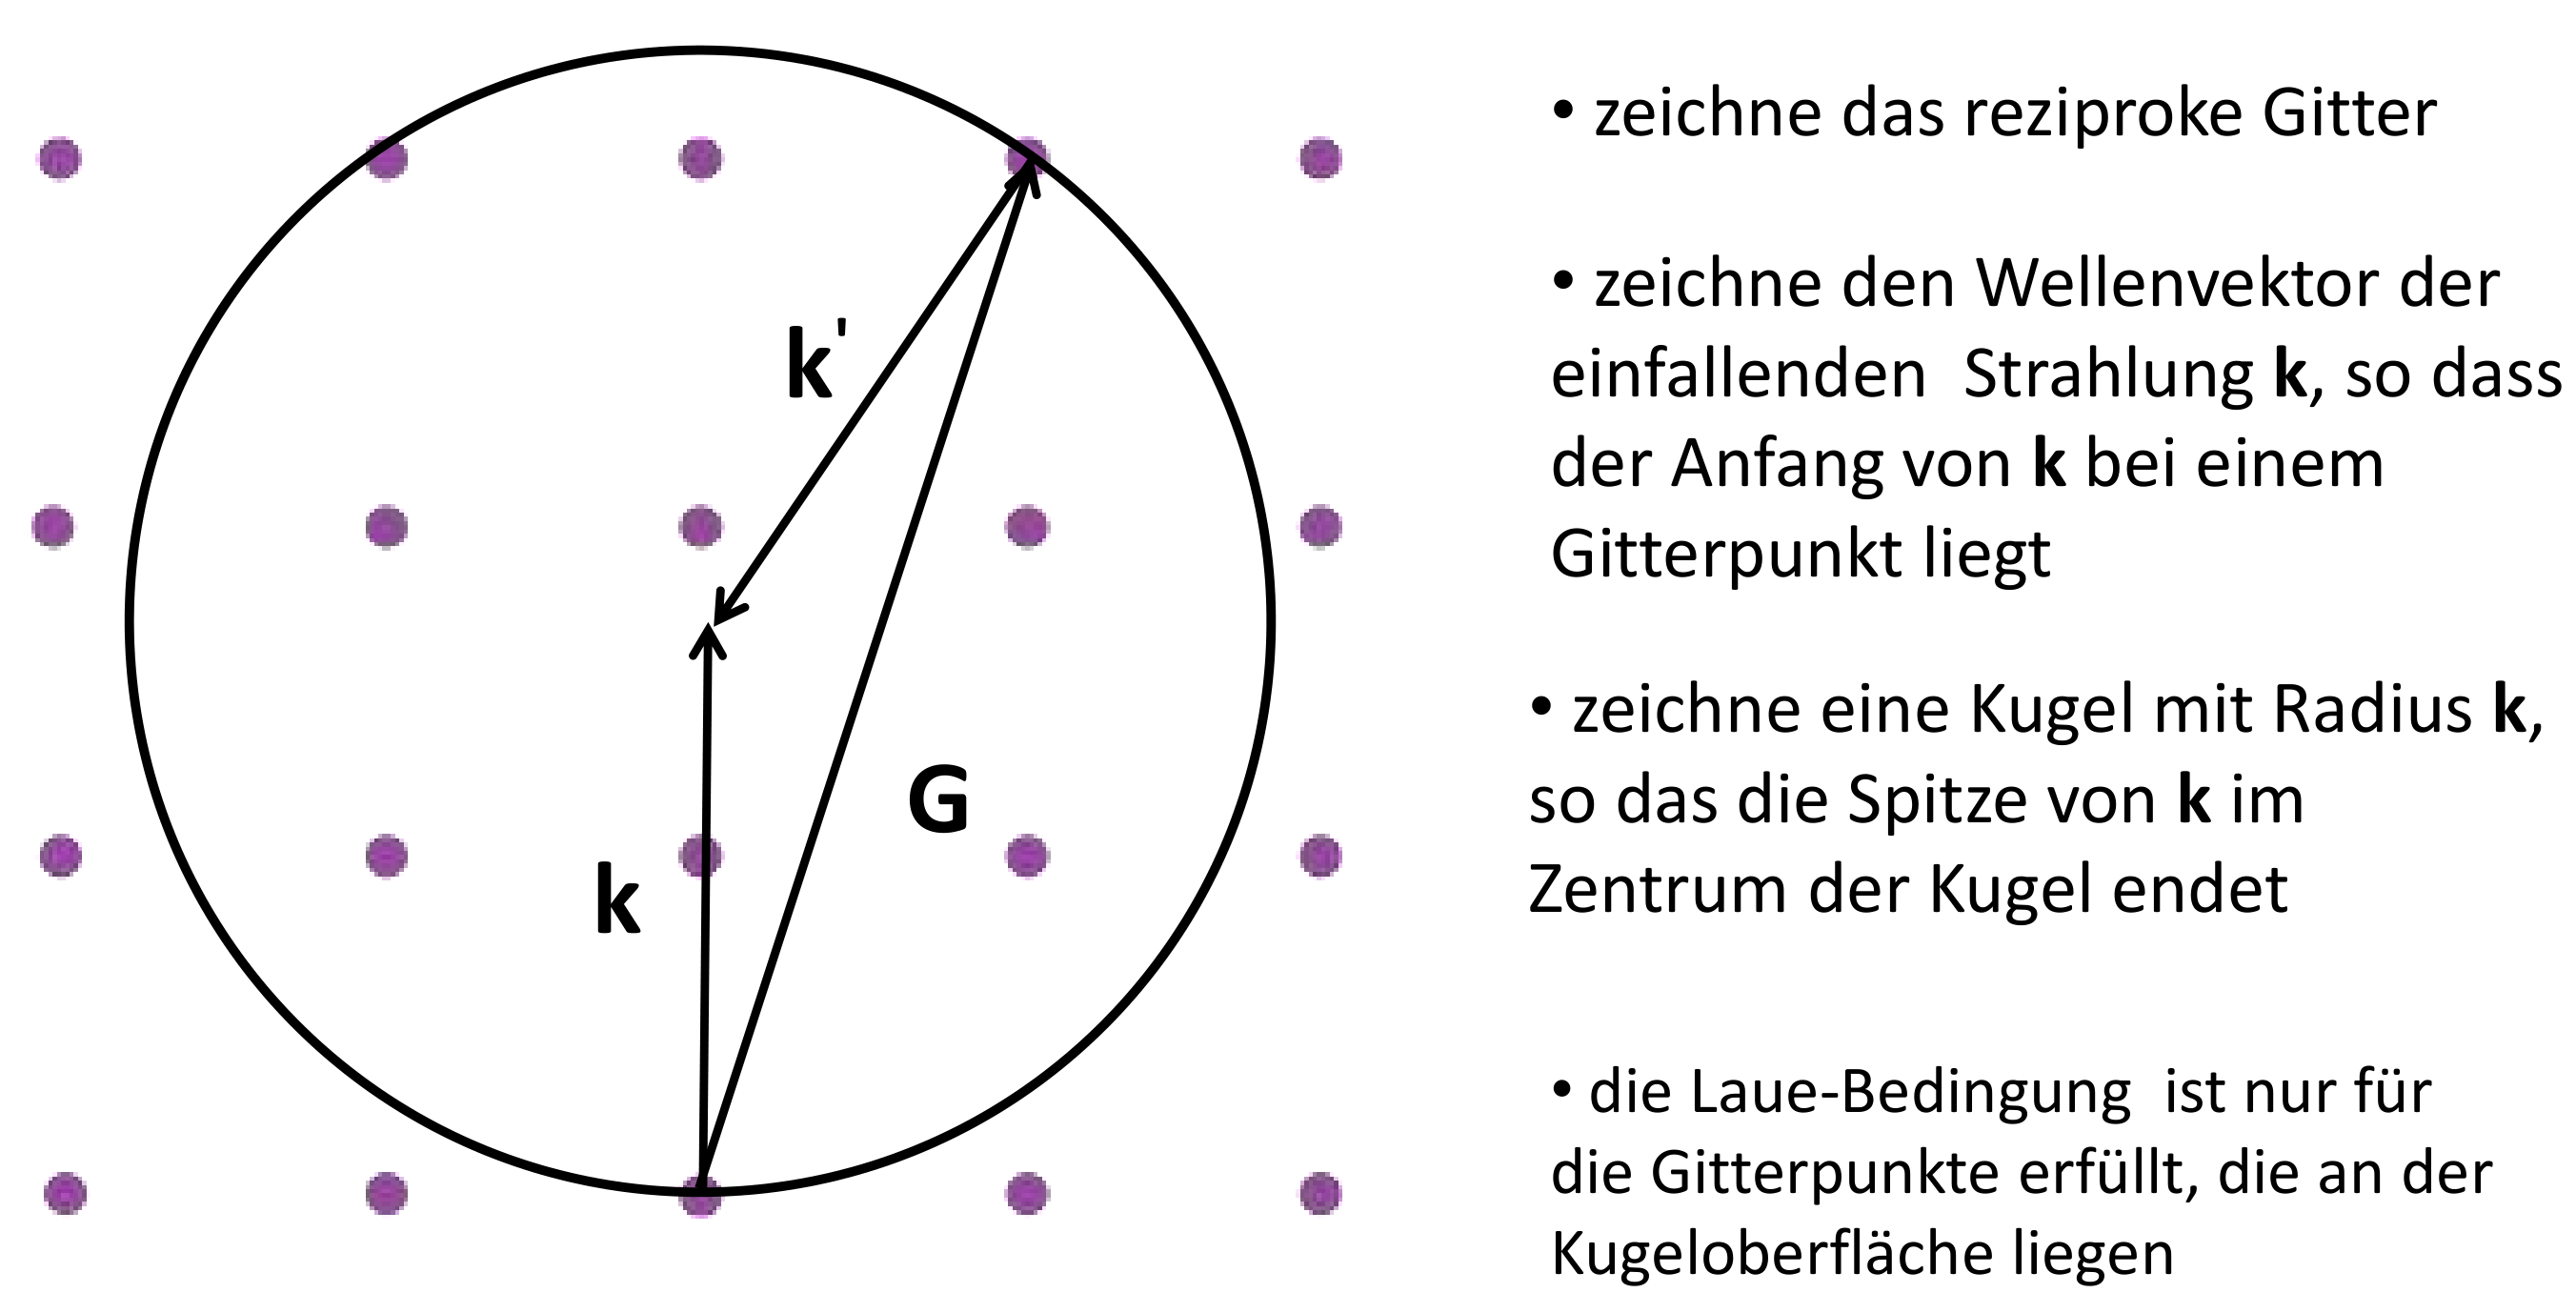
\includegraphics[width=0.8\linewidth]{resources/09-05-2012/Ewald_Konstruktion.png}
        \caption{Ewald-Konstruktion}
    \end{samepage}
\end{figure}

Die Laue-Bedingung ist hierbei nur für die Gitterpunkte erfüllt, die an der Kugeloberfläche liegen. 


\question{Erläutere den Atomfaktor und den Strukturfaktor bei der Röntgenbeugung.}
\label{q:27}

Der Strukturfaktor $S_{hkl}$ bzw. $S_{\vec{G}}$ ist die Fourier-Transformierte $n_{\Vec{G}}$ der Elektronendichte $n(\vec{r})$ über eine Einheitszelle. 
\begin{align}
    S_{\vec{G}} = n_{\vec{G}} = \int_{\text{EZ}} n(\vec{r}) e^{i \vec{G} \vec{r}} d\vec{r} 
\end{align}

\textit{(andere Definition, nicht in Surnev-Folien)} -- Doch, eigentlich schon (siehe 5. Intensität der Beugungsreflexe!) \\
Der Strukturfaktor wird aus den Formfaktoren $f_J(G)$ berechnet werden, welche ebenfalls mit Fourier-Transformation berechnet werden:
\begin{align}
f_J(G) = \int n_J(\vec{r}) e^{i \vec{G} \vec{r}} d\vec{r}
\end{align}
Dabei ist $n_J$ das \textit{Streuvermögen} (z.B. die Elektronendichte) des $J$-ten Atoms.
\begin{align}
S_{\vec{G}} = \sum_j f_j (G) e^{i \vec{G} \vec{r}_j} = \sum_j f_j e^{-2 \pi i (hx_j + ky_j + l z_j)}
\end{align}
wobei $\vec{G}_{hkl} = h\vec{b}_1+k\vec{b}_2+l\vec{b}_3$ der reziproke Gittervektor ist. \\




Der Strukturfaktor ist auch die \textbf{Streuamplitude} pro Einheitszelle:
\begin{align}
S_{h,k,l} = \frac{F_{h,k,l}}{N}
\end{align}
mit der Anzahl an Einheitszellen $N$ und der Streuamplitude:
\begin{align}
    F_{h,k,l} = \int n(\vec{r}) e^{-i \phi(\vec{r})} dV = \int n(\vec{r}) e^{-i \Delta \vec{k} \vec{r}} dV
\end{align}
Für diese Beschreibungen des Strukturfaktors muss die Laue-Bedingung $\vec{G} = \Delta \vec{k} = \vec{k'}-\vec{k}$ erfüllt sein. \bigskip \\

Der \textbf{Atomfaktor} (auch Streufaktor genannt) beschreibt die Beiträge eines einzelnen Atoms zur Streuung von Röntgenstrahlen bzw. das Streuvermögen der einzelnen Basisatome. Er hängt von der Atomart, der Position des Atoms im Kristallgitter und der Wellenlänge der Röntgenstrahlung ab. Der Atomfaktor ist komplex und enthält Informationen über die Elektronendichteverteilung im Atom.

Der Atomfaktor für ein Atom $j$ kann wie folgt definiert werden:

\begin{align}
f_j = \int n_j (\vec{\rho}) e^{-i \vec{G} \vec{\rho}}
\end{align}

Mit kugelsymmetrischen $n(\vec{\rho})$ und $\vec{G} \vec{\rho} = G \rho \cos{\alpha}$ erhält man die Formel
\begin{align}
f = 4 \pi \int_0 ^{\inf} \rho^2 n(\vec{\rho}) \frac{\sin{G \rho}}{G \rho} d\rho
\end{align}

Für eine punktförmige Ladung mit $\vec{\rho} = 0$:
\begin{align}
\frac{\sin{G \rho}}{G \rho} \approx 1 \hspace{1cm} n = \frac{Z}{V} \Rightarrow f = Z
\end{align}
Für kleine Streuwinkel mit $G \approx 0$:
\begin{align}
f = Z
\end{align}

\question{Skizziere die 1. Brillouin Zone eines ebenen Rechteckgitters.}
\label{q:28}

\begin{figure}[H]
    \centering
    \begin{samepage}
        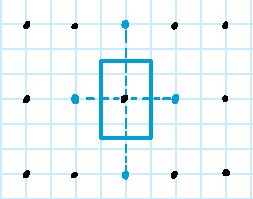
\includegraphics[width=0.4\linewidth]{resources/09-05-2012/BZ1.pdf}
        \caption[1. BZ Rechteckgitter]{1. Brillouin-Zone eines Rechteckgitters}
        \label{fig:BZ1_rechteckgitter}
    \end{samepage}
\end{figure}
\begin{enumerate}
    \item Reziprokes Gitter aufzeichnen
    \item Zellenmittelpunkt wählen
    \item Vom Mittelpunkt in beide Dimensionen den nächstgelegenen Gitterpunkt finden
    \item Mittelpunkt mit diesen Punkten verbinden
    \item Auf den Mittelpunkt der Verbindenden eine Orthogonale zeichnen
\end{enumerate}

\question{Wodurch unterscheiden sich akustische von optischen Phononen?}
\label{q:29}

Ein Phonon ist die elementare Anregung (Quant) des elastischen Feldes. Sie beschreiben die elementare bzw. kollektive Anregungen der Gitterschwingungen eines Festkörpers.
In einem dreidimensionalen Kristall mit $N$ Atomen in der primitiven Basis existieren zu jedem mit der Kristallsymmetrie verträglichen Wellenvektor 
$3N$ mögliche Schwingungsmoden:

\begin{itemize}
    \item Akustische Phononen: Diese Phononen werden auch als Schallquanten bezeichnet und sind die Quanten der Schallwellen, die sich durch das Kristallgitter fortpflanzen.
          Alle Quanten bewegen sich hier in einer Einheitszelle in Phase und haben 3 akustische Moden, wovon eine longitudinal und zwei transversal sind.

          \begin{figure}[H]
            \centering
            \begin{samepage}
                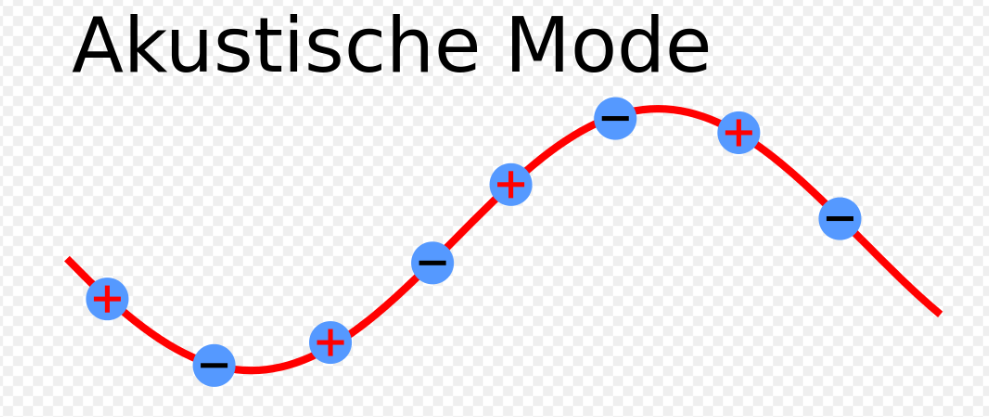
\includegraphics[width=0.8\linewidth]{resources/09-05-2012/akust.PNG}
                \caption[Akustische Transversalwellen Phononen]{Darstellung von akustischen Transversalwellen von Phononen}
                \label{fig:akustische_transversalwellen_phononen}
            \end{samepage}
          \end{figure}

    \item Optische Phononen: Diese Phononen bewegen sich in einer Basis gegenphasig, wodurch es Schwingungsmodi gibt, bei denen entgegengesetzt geladene Untergitter gegeneinander schwingen. 
          Die dabei oszillierenden Dipolmomente können mit Photonen wechselwirken. Oft kommen solche Kopplungen im Infrarotbereich, also der Wärmebewegung in Festkörpern vor.
          Beispiele für solche infrarot-aktiven Gitter sind Ionengitter wie Natriumchloridkristalle.

         \begin{figure}[H]
             \centering
             \begin{samepage}
                 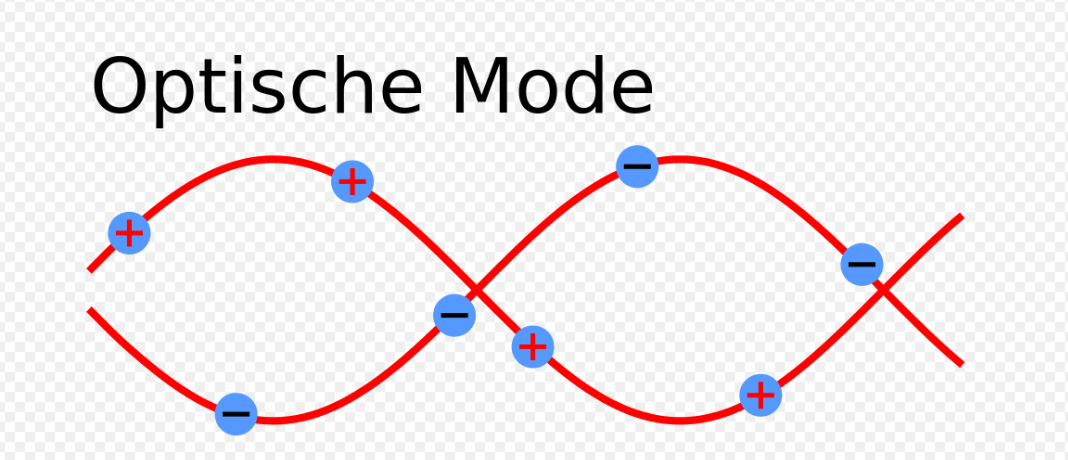
\includegraphics[width=0.8\linewidth]{resources/09-05-2012/opt.PNG}
                 \caption[Optische Wellen Phononen]{Darstellung von optischen Phononen}
                 \label{fig:optische_wellen_phononen}
             \end{samepage}
         \end{figure}

\end{itemize}



\question{Vergleiche die Einstein- und Debye-Modelle der spez. Wärme. Welche Annahme ist im 
Einstein Modell zu einfach?}
\label{q:30}

\begin{figure}[H]  
    \centering
    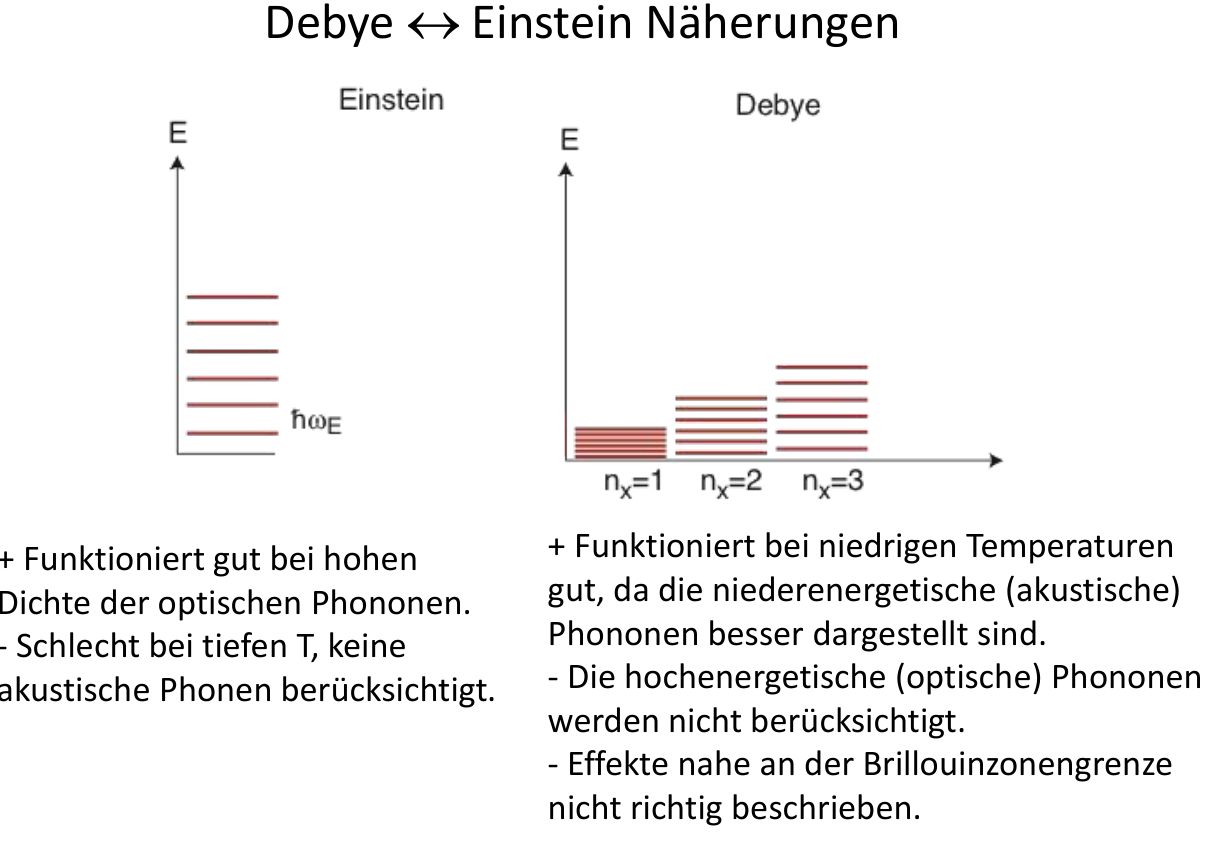
\includegraphics[width=.8\textwidth]{resources/09-05-2012/q30.png}
    \caption{Vergleich zwischen Einstein- und Debye-Modell.}
\end{figure}

Das Einsteinmodell nimmt an, dass alle Atome im Kristall mit der gleichen Frequenz schwingen, zudem werden keine akustischen Phononen berücksichtigt.

\newpage
\section{15. Juni 2015}

\question{Elektronenkonfiguration von \ch{B2} ($Z=5$)}
\label{q:31}

\[\ch{B_2} : (1\sigma_g)^2 ~ (1\sigma_u^*)^2 ~ (2\sigma_g)^2 ~ (2\sigma_u^*)^2 ~ (1\pi_u)^2\]

\begin{figure}[H]
    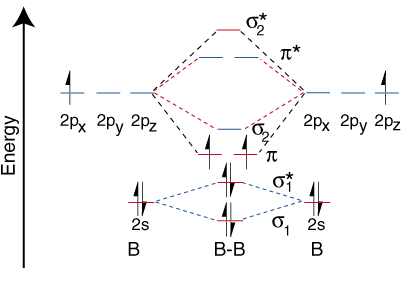
\includegraphics[width=0.8\linewidth]{resources/15-06-2015/b2.PNG}
    \caption{Elektronenkonfiguration von \ch{B2}}
\end{figure}

\question{Arten von Para-Diamagnetismus}
\label{q:32}

\question{Konzept von Bravais Wigner-Seitz Zelle}
\label{q:33}

Die Bravais Wigner-Seitz Zelle ist definiert als die Zelle im Raum, die jedem Gitterpunkt am nächsten 
liegt. Sie hat die folgenden Eigenschaften:
\begin{enumerate}
    \item Symmetrie: Die Zelle ist symmetrisch um den Gitterpunkt, von dem aus sie konstruiert wurde, sie weist alles Symmetrieoperationen, welche im gesamten Gitter vorkommen, auf. 
    \item Ein Gitterpunkt pro Zelle: Die Zelle enthält genau einen Gitterpunkt im Inneren der Zelle. Alle anderen Gitterpunkte des Gitters liegen auf den Seitenflächen der Zelle.
    \item Nächste Nachbarn: Die Zelle teilt den Raum so auf, dass jeder Gitterpunkt seinem nächstgelegenen Nachbarn am nächsten ist.
\end{enumerate}

Konstruktion:
\begin{figure}[H]
    \centering
    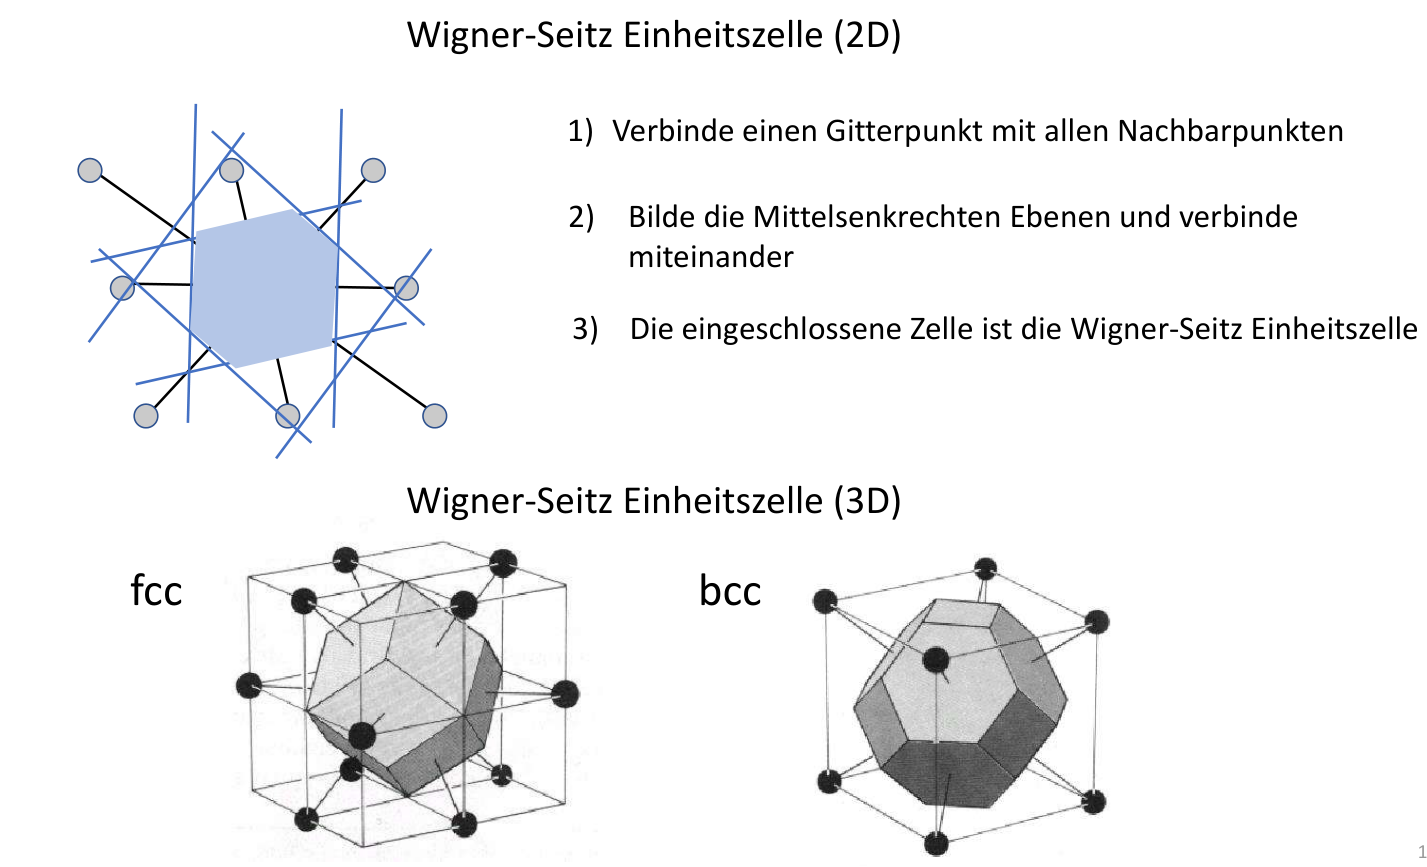
\includegraphics[width=0.8\linewidth]{resources/15-06-2015/q33.png}
    \caption{Konstruktion der Wigner-Seitz Zelle}
\end{figure}

\question{Sp sp2 sp3 Bindungen von mehratomigen Molekülen}
\label{q:34}

\question{Debye-Petit (oder so, irgendwas mit spezifischer Wärme von Elektronen)}
\label{q:35}

\question{Atom/Struktur Faktor}
\label{q:36}

\question{Zustandekommen von Energiebändern und Bandlöchern}
\label{q:37}

\textbf{TL;DR} Braggreflexion ist die Ursache für Energiebandlücken, da bei Braggreflexion keine Wellenartigen Lösungen der Schrödingergleichung existieren.
Energiebänder sind die Resultate der Energiebandlücken.

\textbf{TS;WR} Freie $e^-$ mit kontinuierlichen Energien besitzen Wellenfunktionen von der Form $\psi_{k}(\vec{r}) = exp(i\vec{k}\vec{r})$

Man nehme einen eindimensionalen Kristall mit Gitterkonstante $a$.
Die Braggbedingung\\$\left(\vec{k} + \vec{G}\right)^2 = k^2$ für Beugung eines Wellenvektors $\vec{k}$ ergibt sich in 1D zu
\begin{equation}
    k = \frac{\pm G}{2} = \frac{\pm n \pi}{a}
\end{equation}
wobei $G = 2\pi n/a$ ein reziproker Gittervektor ist und $n \in \mathbb{N}$.

Bei solchen $k$ (hier mit $n=1$) überlagert sich die Wellenfunktion $exp(\pm i \pi x / a)$ eines Wandernden $e^-$ mit seiner Bragg Reflektierten.
Mit $exp(\pm i \pi x / a) = cos(\pi x/a) \pm i sin(\pi x/a)$ erhält man eine symmetrische stehende Welle
\begin{equation}
    \psi(+) = exp( i \pi x / a) + exp(- i \pi x / a) = 2cos(\pi x/a)
\end{equation}
und eine antisymmetrische
\begin{equation}
    \psi(-) = exp( i \pi x / a) - exp(- i \pi x / a) = 2 i sin(\pi x/a)
\end{equation}
ähnlich wie in den Hybridisierungsorbitalen einer Doppelbindung.
Die Aufenthaltswahrscheinlichkeiten $\left|\psi(\pm)\right|^2$ in Kombination mit den Potentialen der Atomkerne (Abb.a)) zeigen, dass die symmetrische Wellenfunktion $\psi(+)$ mehr negative Ladung an die positiven Ionen zieht und dadurch geringere potentielle Energie besitzt, als eine laufende Welle und $\psi(-)$ eine höhere potentielle Energie als eine laufende Welle besitzt.
\begin{figure}[H]
    \centering
    \begin{subfigure}[c]{0.4\textwidth}
        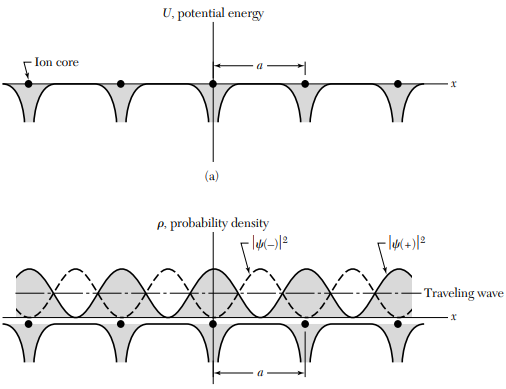
\includegraphics[width=\linewidth]{resources/15-06-2015/q37a.png}
        \caption{}
    \end{subfigure}%
    \begin{subfigure}[c]{0.4\textwidth}
        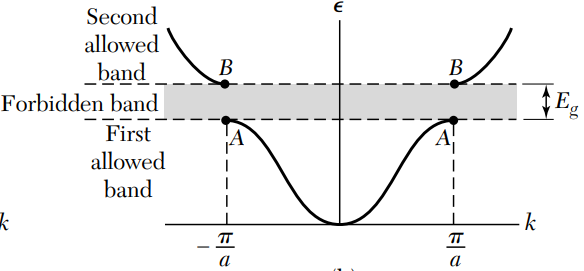
\includegraphics[width=\textwidth]{resources/15-06-2015/q37b.png}
        \caption{}
    \end{subfigure}% 
    \caption{
        a) Aufenthaltswahrscheinlichkeiten $\left|\psi(\pm)\right|^2$ und für laufende Wellen zusammen mit der Potentiellen Energie einer negativen Ladung um die Kerne.
        b) Energie plot mit Bandlücke.
        }
\end{figure}

\question{Zusammenhang zwischen Gitterebene und Vektoren im reziproken Gitter}
\label{q:38}

Siehe \aqref{4}.

\question{Statische Abschirmung des Elektronengases}
\label{q:39}

\question{Einstein-Debye Unterschiede und falsche Annahmen}
\label{q:40}
\textbf{Einstein-Näherung} 
\begin{itemize}
    \item Annahme: alle Atome im Kristall schwingen mit der gleichen Frequenz $\omega$ = $\omega_E$, wobei $\omega_E$ die Frequenz der optischen Moden darstellt. 
    \item lässt sich nur auf optische Moden anwenden (nicht auf akkustische!)
    \item funktioniert gut bei hoher Dichte der optischen Phononen und liefert richtiges 
    Hochtermperaturlimit nach Dulong-Petit-Gesetz
    \item funktioniert schlecht bei tiefen Temperaturen und liefert ungenaues Limit für niedrige Temperaturen
    \item Falsche Annahme: akkustische Moden werden nicht berücksichtigt und alle harmonischen Oszillatoren im Festkörper würden mit einheitlicher Frequenz schwingen.
\end{itemize}

\textbf{Debye-Näherung} 
\begin{itemize}
    \item Annahme: 
        \begin{itemize}
            \item Vielzahl möglicher Frequenzen und Ausbreitungsgeschwindigkeit $v_i$ von Wellen/Phononen. 
            \item Lineare Dispersion $\omega_i=v_ik$ 
        \end{itemize}
    \item berücksichtigt nur akkustische Moden
    \item funktioniert gut bei niedrigen Temperaturen, da niederenergetische (akkustische) Phononen besser dargestellt sind 
    \item liefert korrektes Limit für hohe und tiefe Temperaturen
    \item Falsche Annahme: optische Phononen werden nicht berücksichtigt und Effekte nahe der Brillouinzonengrenze werden nicht richtig beschrieben
\end{itemize}

\begin{figure}[H]
 \centering
 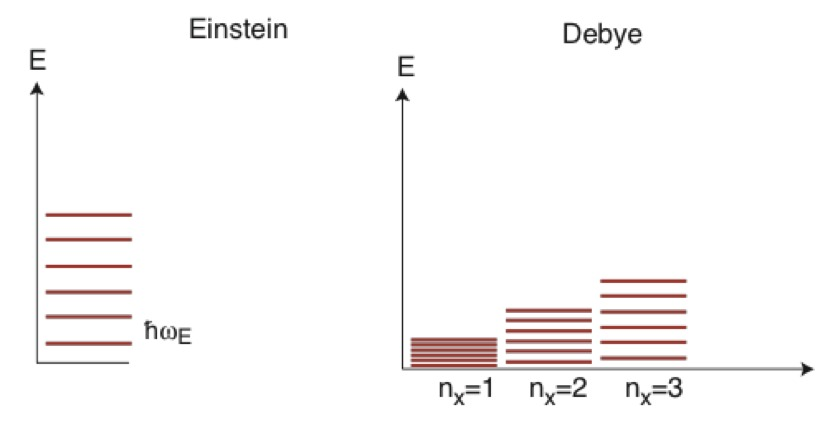
\includegraphics[width=0.6\textwidth]{resources/15-06-2015/Einstein_Debye.jpeg}
 \caption{Einstein- vs. Debye-Modell}
 %\label{}
\end{figure}
\newpage
\section{16. März 2012}

\question{Diskutieren der unterschiedlichen Überlegungen in der Valenzbindungsnäherung (VB) und in der Molekularorbitalnäherung (MO) zur Beschreibung der Molekülbindung in einem 2-atomigen Molekül}
\label{q:41}

\textbf{VB-Näherung}
\begin{itemize}  
    \item liefert KEINE Details über Molekülorbitale
    \item im Grundzustand können zwei Elektronen mit $\uparrow \downarrow$ Spins untergebracht werden
    \item zwei \textbf{lokalisierte} Elektronen um Kerne A und B
    \item beide Elektronen werden betrachtet, sodass für beide Wahrscheinlichkeitsamplituden $\psi_1$ und $\psi_2$ ein Produktansatz der Atomorbitale notwendig ist
    \item Besetzung des Molekülorbitals wird mit Linearkombination von $\psi_1$ und $\psi_2$ durch Pauli-Prinzip erzwungen
    \item \textbf{$e^-$ lokalisiert}
\end{itemize}
2 $e^-$ werden zugleich beschrieben:
\[\psi_1(\vb{r_1},\vb{r_2}) = c_1 \phi_A(\vb{r_1}) \cdot \phi_B(\vb{r_2})\]
\[\psi_2(\vb{r_1},\vb{r_2}) = c_2 \phi_A(\vb{r_2}) \cdot \phi_B(\vb{r_1})\]
und danach symmetrisch/antisymmetrisch kombiniert: 
\[\psi_{\text{sym}} (\vb{r_1},\vb{r_2}) = \psi_1(\vb{r_1}) + \psi_2(\vb{r_2})\]
\[\psi_{\text{asym}}(\vb{r_1},\vb{r_2}) = \psi_1(\vb{r_1}) - \psi_2(\vb{r_2})\]

\noindent
\textbf{MO-Näherung}
\begin{itemize}
    \item erklärt Paarung von Elektronen durch Überlappung von Orbitalen ($\sigma$- und $\pi$-Bindungen)
    \item basiert auf bindenden und antibindenden Molekülorbitalen
    \item erklärt die Hybridisierung der Orbitale
    \item ein Elektron betrachtet, dass sich in $\phi_A$ als auch in $\phi_B$ aufhalten kann, sodass für dieses ein Molekülorbital-Ansatz notwendig ist (wobei $\phi_A$ und $\phi_B$ atomare Wellenfunktionen)
    \item für Besetzung des Molekülorbitals mit zwei Elektronen wird Produktansatz verwendet
    \item \textbf{$e^-$ delokalisiert}
\end{itemize}
$e^-$ werden einzeln beschrieben als Linearkombination der Atomorbitale (LCAO):
\[\psi_i(\vb{r}_i) = c_1 \cdot \phi_A(\vb{r}_i) + c_2 \cdot \phi_B(\vb{r}_i)\]
2 $e^-$ werden mittels Produktansatz kombiniert:
\[\psi(\vb{r}_1,\vb{r}_2) = \psi_1(\vb{r}_1) \cdot \psi_2(\vb{r}_2) \]

\question{Skizzieren der bindenden und antibindenden Wellenfunktionen in einem homonuklearen 2-atomigen Molekül}
\label{q:42}
\begin{figure}[H]
    \centering
   \begin{minipage}[b]{.4\linewidth} % [b] => Ausrichtung an \caption
      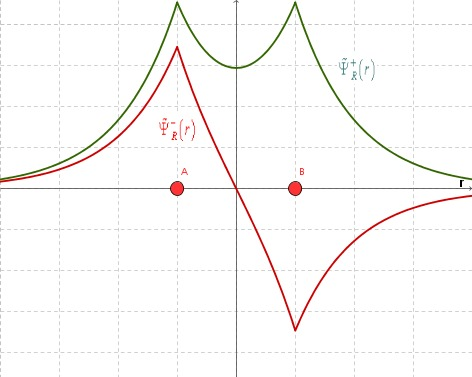
\includegraphics[width=\linewidth]{resources/16-03-2012/sym_und_antisymm_Wellenfunktion.jpeg}
      \caption{\textbf{Wellenfunktionen} symmetrische (bindend, grün) und antisymmetrische (antibindende, rot) Wellenfunktion}
   \end{minipage}
   \hspace{.1\linewidth}% Abstand zwischen Bilder
   \begin{minipage}[b]{.4\linewidth} % [b] => Ausrichtung an \caption
      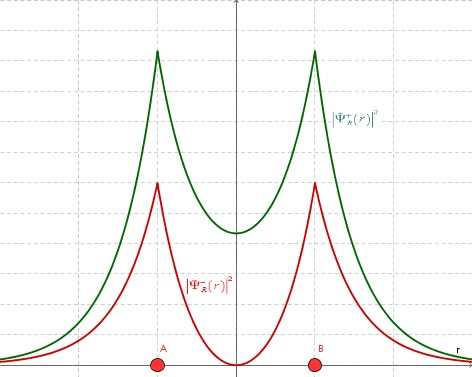
\includegraphics[width=\linewidth]{resources/16-03-2012/Wahrscheinlichkeitsdichten.jpeg}
      \caption{Wahrscheinlichkeitsdichten der symmetrischen (bindend, grün) und antisymmetrischen (antibindende, rot) Wellenfunktion}
   \end{minipage}
\end{figure}

\question{Diskutieren des Schwingungsrotationsspektrums eines 2-atomigen Moleküls}
\label{q:43}

\begin{itemize}
    \item Spektren zweiatomiger Moleküle entstehen durch Rotations- und Schwingungsübergänge
    \item im realen Molekül führen Kerne um Gleichgewichtsabstand $R_e$ Schwingungen aus, sodass sich Kernabstand $R$ während Rotation des Moleküls ändert
    \item \textbf{Rotationsspektren}
        \begin{itemize}
            \item entstehen durch Absorption des Moleküls im Infrarot-Bereich
            \item durch Energieaufnahme kommt es zu Strahlungsübergänge zwischen den Rotationszuständen
            \item in einfachster Näherung wird Molekül als \textbf{starrer Rotator} betrachtet, der sich mit konstantem Kernabstand $R=R_e$=const um Schwerpunktachse dreht. Rotationsenergie $E_{rot}$ ,als Termwert $F_{rot}$, hat bei $R=R_e$ diskrete Werte, siehe \ref{RotEnergie_starr} \ref{Termwert_RotE}. Die Abstände der Energieniveaus $\Delta E_{rot}$ nehmen linear zu, siehe \ref{Abstaende_Eniveaus_starr}.

                \begin{equation}
                E_{rot} = \frac{J(J+1)\hbar^2}{2MR_e^2}
                \label{RotEnergie_starr}
                \end{equation}

                \begin{equation}
                F_{rot} =B_eJ(J+1)=\frac{\hbar}{4\pi cMR_e^2}J(J+1) \hspace{5mm} \left[cm^{-1}\right]
                \label{Termwert_RotE}
                \end{equation}

                \begin{equation}
                \Delta E_{rot}=E_{rot}(J+1)-E_{rot}=\frac{(J+1)\hbar^2}{I}
                \label{Abstaende_Eniveaus_starr}
                \end{equation}

            \item beim \textbf{nicht-starren Rotator} (Zentrifugalkraft berücksichtigt) besteht elastische Bindung zwischen Atomen mit Federkonstante k. Der Kernabstand vergrößert sich von $R_e$ auf $R$, dabei wird das Trägheitsmoment $I=MR^2$ größer und die Rotationsenergie $F_{rot}$ kleiner, siehe \ref{RotE_nichtstarr}. Die Spektrallinien rücken mit steigender Rotationsquantenzahl J=0,1,2,... weiter auseinander. Im Vergleich zum starren Rotator liegen sie jedoch näher beisammen.
                \begin{equation}
                   F_{rot}=B_eJ(J+1)-D_eJ^2(J+1)^2+...
                   \label{RotE_nichtstarr}
                    \end{equation}
    \begin{figure}[H]
    \centering
   \begin{minipage}[b]{.3\linewidth}
      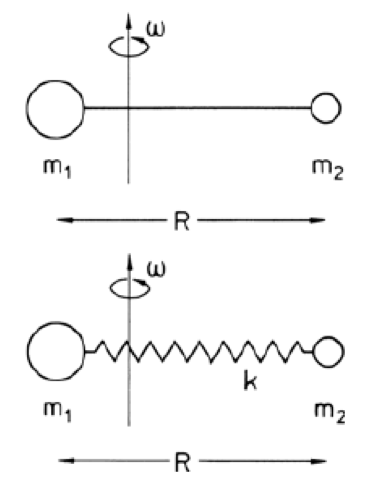
\includegraphics[width=\linewidth]{resources/16-03-2012/StarrervsnichtstarrerRotor.png}
      \caption{starrer Rotor vs nicht starrer Rotor}
   \end{minipage}
   \hspace{.1\linewidth}
   \begin{minipage}[b]{.3\linewidth} 
      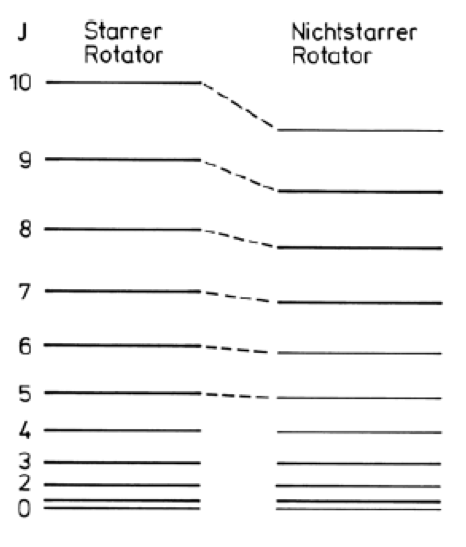
\includegraphics[width=\linewidth]{resources/16-03-2012/2starrervsnichtstarrerrotos.png}
      \caption{Übergänge starrer vs nicht starrer Rotor}
   \end{minipage}
    \end{figure}
                
        \end{itemize}

    \item \textbf{Rotationsschwingungsspektren}
        \begin{itemize}
            \item entstehen durch Absorption/Emission des Moleküls im Infrarot-Bereich, wobei Rotation und Schwingung gleichzeitig verändert werden
            \item jede Bande des Rotationsschwingungsspektrums entspricht einem Schwingungsübergang
            \item in einfachster Näherung bilden schwingende Atome des Moleküls einen \textbf{harmonischen Oszillator} mit diskreten Energie $E_{vib}$, siehe \ref{EVib_harmonisch}, und gleich großen Energieabstände $\Delta E_{vib}$, siehe \ref{EVib_Abstaende}. Potential kann durch Parabelpotential angenähert werden.

                \begin{equation}
                    E_{vib}(\nu)=(\nu+\frac{1}{2})\hbar \omega
                \label{EVib_harmonisch}
                \end{equation}

                \begin{equation}
                \Delta E_{vib}=\hbar \omega
                \label{EVib_Abstaende}
                \end{equation}

            \item bei Näherung als \textbf{anharmonischer Oszillator} rücken die Enrgieniveaus mit zunehmender Schwingungsquantenzahl $\nu$=0,1,2,... näher zusammen und konvergieren gegen Dissoziationsenergie des Moleküls. Potential kann durch Morse-Potential (\autoref{eq:morse_potential}) angenähert werden.
            \begin{equation}
                \label{eq:morse_potential}
                U(r) = U_0 \left( e^{-2(r-r_0)/a} - 2e^{-(r-r_0)/a} \right)
            \end{equation}
        \end{itemize}

\end{itemize}


\begin{figure}[H]
    \centering
   \begin{minipage}[b]{.4\linewidth}
      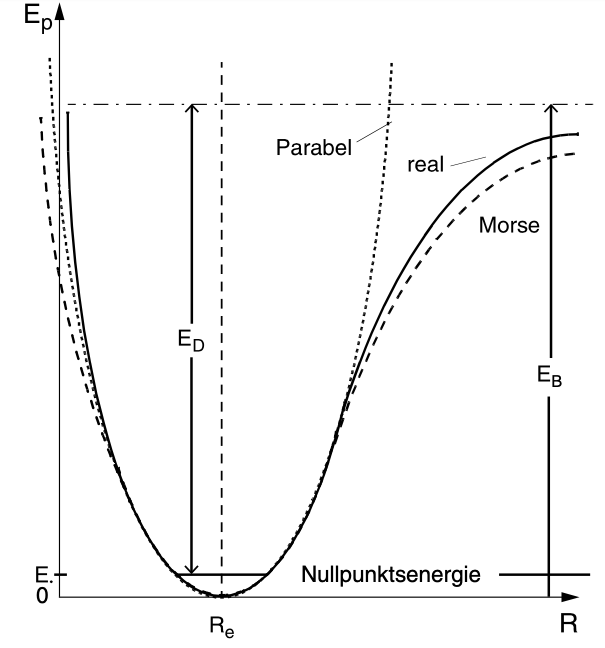
\includegraphics[width=\linewidth]{resources/16-03-2012/Vergleich_ParabelMorseReal.png}
      \caption{Vergleich zwischen Parabel-, Morse- und realen Potentials}
   \end{minipage}
   \hspace{.1\linewidth}
   \begin{minipage}[b]{.4\linewidth} 
      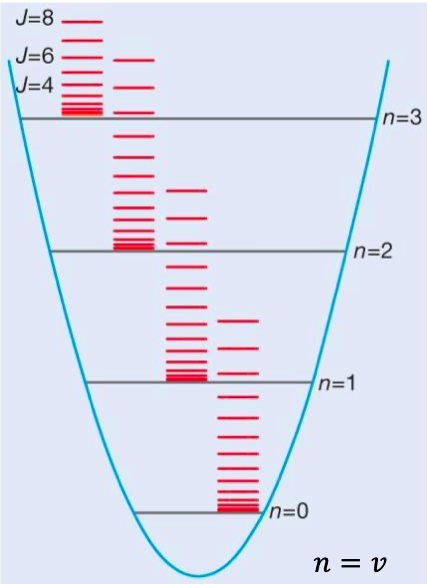
\includegraphics[width=0.8\linewidth]{resources/16-03-2012/SchwingugsRotatioinsspektrum.png}
      \caption{Darstellung der Rotations- und Schwingungsniveaus, jedem Schwingungsniveau ist Reihe von Rotationsniveaus zugeordnet}
   \end{minipage}
    \end{figure}


\question{Diskutiere die chemische Bindung im \ch{Li2}-Molekül}
\label{q:44}

Jedes Lithium-Atom liefert jeweils 3 Elektronen, insgesamt also 6 Elektronen. 
Somit sind die Molekülorbitale
\[\ch{Li2} : (1\sigma_g)^2 ~ (1\sigma_u^*)^2 ~ (2\sigma_g)^2\]
besetzt. 
Da das $(2\sigma_g)$-Orbital als höchstes besetzt ist, handelt es sich um eine stabile Bindung. 
Es gibt ein bindendes Elektronenpaar und daher handelt es sich um eine kovalente Bindung.

\textbf{Energie-Orbital-Diagram:} Am besten noch ein Energieniveau-Orbital-Diagramm zeichnen, um die Bindung zu verdeutlichen. Dann kann man argumentieren, dass die Bindung stabil ist, weil das $(2\sigma_g)$-Orbital als höchstes besetzt ist und somit die Energie des Moleküls minimiert wird.

\question{Was versteht man unter dem Franck-Condon-Prinzip? Diskutiere die Intensität von Schwingungsbänden in einem Molekülspektrum bei einem elektronischen Übergang anhand des Franck-Condon-Prinzips.}
\label{q:45}

Siehe \aqref{25}.

\question{Wodurch unterscheidet sich ein fcc Gitter von einem hcp?}
\label{q:46}

fcc -- face centered cubic, hcp -- hexagonal close-packed

\begin{enumerate}
    \item Anordnung der Atome: Im fcc-Gitter sind die Atome auf den Eckpunkten eines Würfels sowie in den Zentren der sechs Flächen platziert. Im hcp-Gitter sind die Atome hexagonal angeordnet.
    \item Einheitszelle: Im fcc-Gitter ist die Einheitszelle ein Würfel, jeder Eckpunkt enthält ein Atom. Im hcp-Gitter ist die Zelle ein hexagonales Prisma, jede Basisebene enthält ein Atom.
    \item Schichtstruktur: Im fcc-Gitter gibt es \textbf{ABCABC}-Schichten. Im hcp-Gitter sind die Schichten \textbf{ABAB}-angeordnet.
    \item Komprimierung: Im fcc-Gitter beträgt $a:c = \sqrt{2}:1$. Im hcp-Gitter beträgt $a:c = \sqrt{3}:2$.
    \item Bepackungsdichte: In beiden Gittern beträgt die maximale Bepackungsdichte 0,74.
\end{enumerate}

\question{Erläutere den Atomfaktor und den Strukturfaktor bei der Röntgenbeugung.}
\label{q:47}

Siehe \aqref{27}.

\question{Skizziere die 1. Brillouin-Zone eines ebenen Parallelogrammgitters.}
\label{q:48}

Zur Erklärung der Konstruktion siehe \aqref{28}.
\begin{figure}[H]
    \centering
    \begin{samepage}
        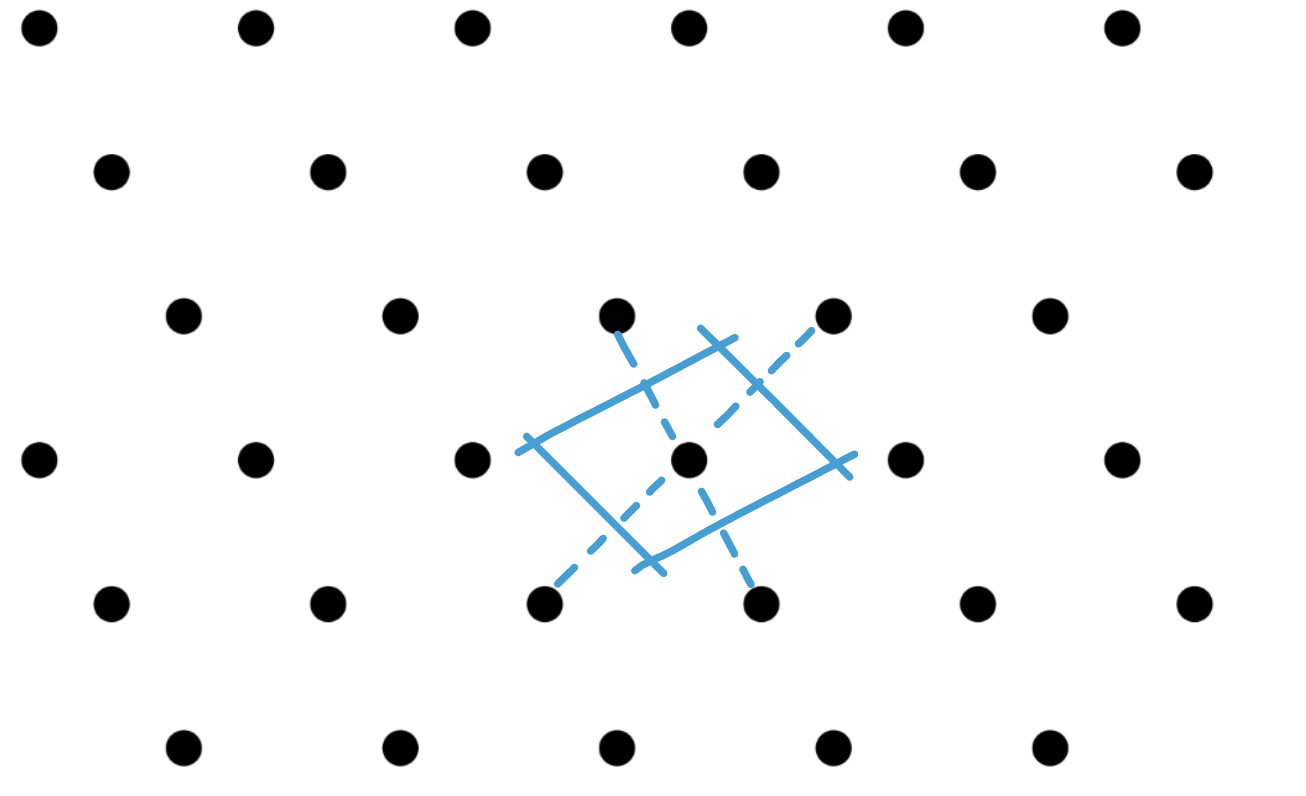
\includegraphics[width=0.4\linewidth]{resources/16-03-2012/BZ1.png}
        \caption[BZ1 Parallelogrammgitter]{1. Brillouin-Zone eines ebenen Parallelogrammgitters}
        \label{fig:BZ1_Parallelogrammgitter}
    \end{samepage}
\end{figure}

\question{Wodurch unterscheidet sich die Dispersionsrelation der Phononen eines primitiven kubischen Gitters von jener eines \ch{CsCl}-Gitters.}
\label{q:49}

\textbf{TL;DR:} Bei primitiv kubischem Gitter haben alle Atome die gleiche Masse $M_n = M$.
Es kommt daher nur zu einer Bewegungsgleichung und in folge nur zu einer Lösung für die Dispersionsrelation $\omega(\vec{k})$.
Dahingegen werden beim \ch{CsCl} Gitter zwei Bewegungsgleichungen benötigt, welche zwei Lösungen für die Dispersionsrelation besitzen mit unterschiedlichen Energien.
Die Lösung mit geringerer Energie beschreibt akustische Phononen und die Lösung mit höherer Energie optische Phononen.

\textbf{TS;WR:} Die Unterschiede können gut durch die Herleitung eines eindimensionalen Kristalls gezeigt werden:\\
\begin{minipage}[t]{0.44\textwidth}
    \centering
    \begin{figure}[H]
        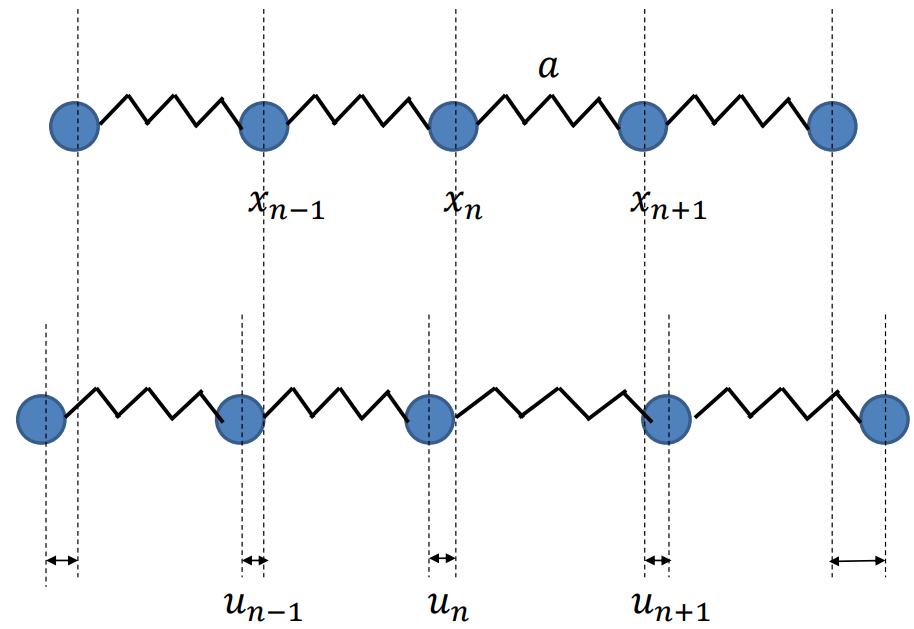
\includegraphics[width=0.7\linewidth]{resources/16-03-2012/q49_same_mass.png}
    \end{figure}
    Ausgehend von der Auslenkung $u_n$ des Atom $n$ aus der Ruhelage $x_n$ und vom Hook'schen Gesetz die Kraft $F_n$ auf Atom $n$ die aus Federverbindung mit Nachbarn resultiert:
    \begin{align*}
        u_n &= x - x_n\\
        F_n &= \sum_{p} C \left(u_{n+p} - u_n\right)
    \end{align*}
    Die Bewegungsgleichung $F_n = M \frac{d^2 u_n}{dt^2}$ ergibt sich zu:
    \begin{align*}
        M \ddot{u}_n &= C\left(u_{n+1} - u_n\right) + C\left(u_{n-1} - u_n\right)\\
        &= C\left(u_{n+1} + u_{n-1} - 2u_n\right)
    \end{align*}
    Als Lösungsansatz der DGL werden logischerweise Wellen verwendet:
    \begin{align*}
        u_n &= U_0 exp(-ikx_n)exp(-iwt)\\
            &= U_0 exp(-ikn\cdot a)exp(-iwt)
    \end{align*}
    Durch einsetzen und vereinfachen ergibt sich:
    \begin{align*}
        -M \omega^2 u_n &= C\left[exp(ika) + exp(-ika) - 2\right] u_n\\
        \rightarrow \omega(k) &= 2 \sqrt{\frac{C}{M}} \abs{sin\left(\frac{ka}{2}\right)}
    \end{align*}
    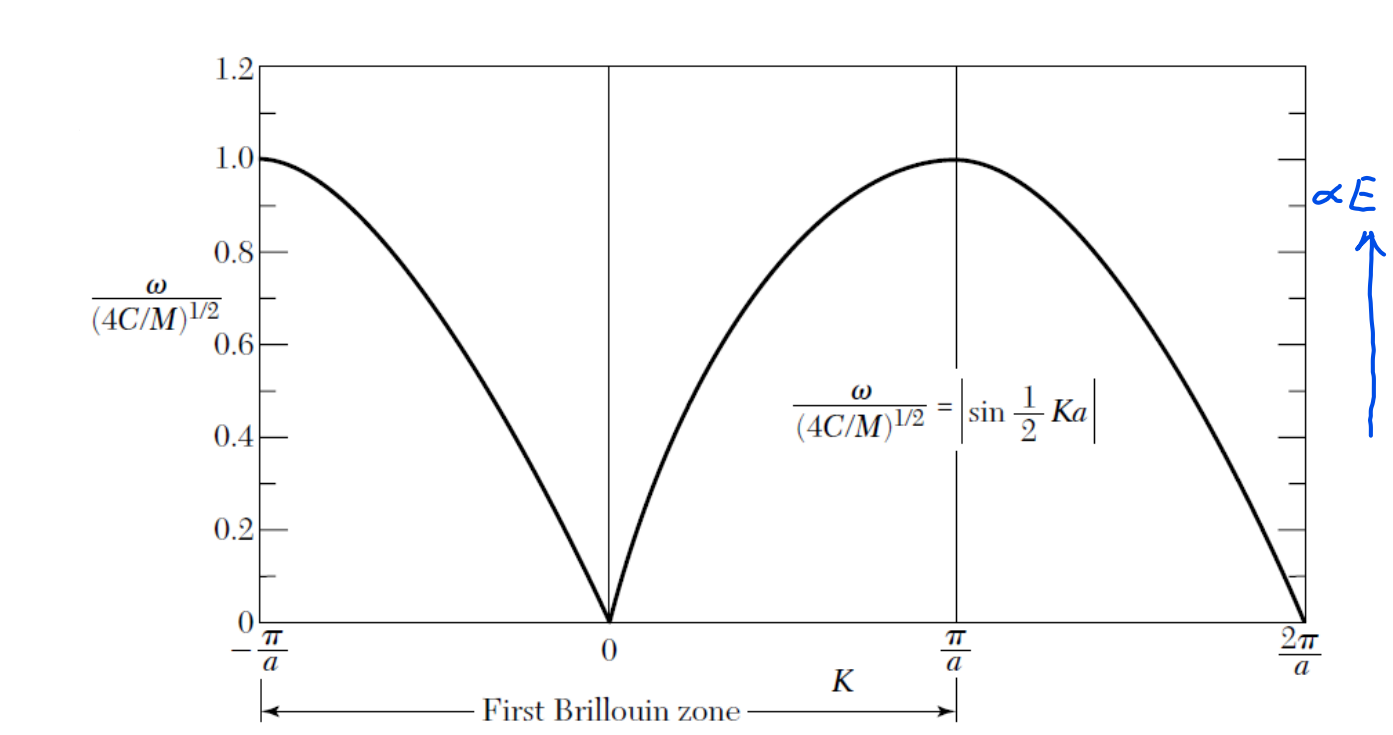
\includegraphics[width=0.9\linewidth]{resources/16-03-2012/q49_same_mass_disp.png}

\end{minipage}
\begin{minipage}[t]{0.5\textwidth}
    \centering
    \begin{figure}[H]
        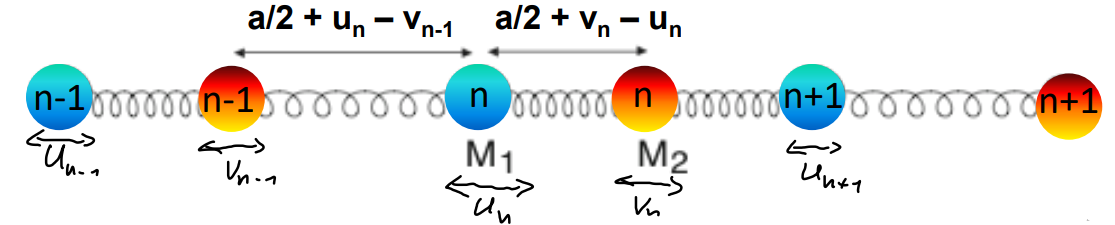
\includegraphics[width=0.9\linewidth]{resources/16-03-2012/q49_diff_mass.png}
    \end{figure}
    Achtung $a$ ist Abstand zwischen den Ruhepositionen gleich schwerer Atome (Einheitszelle).
    Bewegungsgleichungen:
    \begin{align*}
        M_1 \ddot{u}_n &= C\left(v_{n+1} + v_{n-1} - 2u_n\right)\\
        M_2 \ddot{v}_n &= C\left(u_{n+1} + u_{n-1} - 2v_n\right)
    \end{align*}
    Ansätze:
    \begin{align*}
        u_n &= U_0 exp\left(-ikn\cdot a\right)exp(-iwt)\\
        v_n &= V_0 exp\left(-ik\left[n-\frac{1}{2}\right]\cdot a\right)exp(-iwt)
    \end{align*}
    Einsetzen ergibt:
    \begin{align*}
        - M_1 \omega^2 U_0 &= 2CV_0 cos \left(\frac{ka}{2}\right) - 2CU_0\\
        - M_2 \omega^2 V_0 &= 2CU_0 cos \left(\frac{ka}{2}\right) - 2CV_0
    \end{align*}
    Durch multiplizieren (glaub ich) der beiden Gleichungen kommt man auf:
    \begin{align*}
        - M_1M_2\omega^4 - 2C \left(M_1 + M_2\right) \omega^2&\\
        + 4C^2 sin^2\left(\frac{ka}{2}\right)& = 0
    \end{align*}
    \begin{align*}
        \omega^2 &= C \left(\frac{1}{M_1} + \frac{1}{M_2}\right) \pm \sqrt{\left(\frac{1}{M_1} + \frac{1}{M_2}\right)^2} \\
        &\overline{-\frac{4}{M_1 M_2}sin^2\left(\frac{ka}{2}\right)}
    \end{align*}
    $\pm \rightarrow$ 2 Disp.rel. (Herleitung $\omega_{\pm}$ in Folien 7. Dynamik des Kristallgitters S.12-16).
    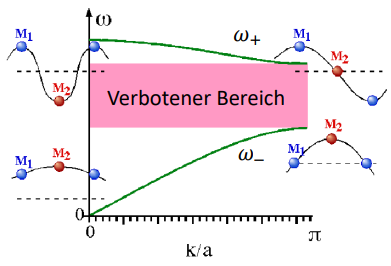
\includegraphics[width=0.7\linewidth]{resources/16-03-2012/q49_diff_mass_disp.png}
\end{minipage}

\question{Vergleiche die Einstein- und Debye-Modelle der spez. Wärme. Welche Annahme ist im Einstein Modell zu einfach?}
\label{q:50}

Siehe \aqref{40}.

\newpage
\section{24. März 2015}

\question{Franck-Condon-Prinzip und Intensität der Übergänge}
\label{q:51}

Siehe \aqref{25}.

\question{Diskutiere die Elektronenkonfiguration von \ch{N2}.}
\label{q:52}

\[\ch{N_2} : (1\sigma_g)^2 ~ (1\sigma_u^*)^2 ~ (2\sigma_g)^2 ~ (2\sigma_u^*)^2 ~ (1\pi_u)^4 ~ (3\sigma_g)^2\]
14 Elektronen werden auf die $\pi$- und $\sigma$-Bindungen aufgeteilt. Achtung: Die Reihenfolge der $1\pi$- und der $3\sigma$-Orbitale kann variieren. Die unterschiedliche Reihenfolge dieser Orbitale kommt durch eine Mischung der s- und p-Atomorbitale zustande: Eine solche kann vorkommen, wenn der energetische Unterschied zwischen dem 2s- und dem 2p-Orbital der Atome klein genug ist (N$_2$ bildet genau die Grenze, bis zu der die Bildung dieser Mischung möglich ist). Dadurch wird zwar das $2\sigma_g$-Orbital stärker bindend, das $3\sigma_g$ wird jedoch schwächer bindend. Dadurch ist das $1\pi_u$-Orbital energetisch günstiger als das $3\sigma_g$ (\autoref{fig:q52}). Ist der (energetische) Abstand zwischen den s- und p-Atomorbitalen groß genug, so kann die Mischung der Orbitale vernachlässigt werden.

\begin{figure}[H]
    \centering
    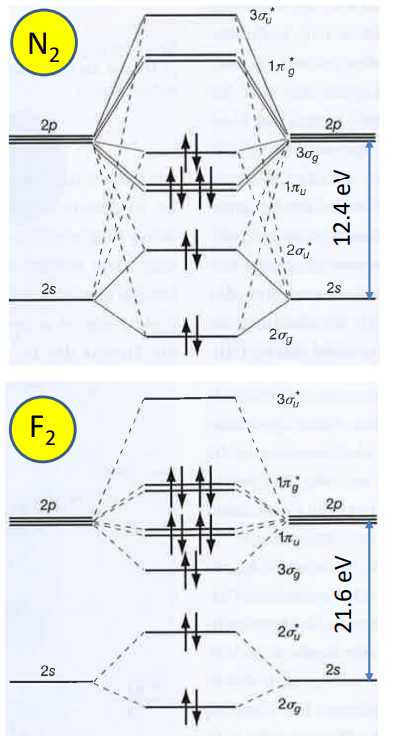
\includegraphics[width=.4\textwidth]{resources/24-03-2015/N2-F2.png}
    \caption{Elektronische Struktur von N$_2$ und F$_2$.}
    \label{fig:q52}
\end{figure}


\question{Diskutiere die Van der Waals Wechselwirkung und das Lennard-Jones Potential.}
\label{q:53}

Befindet sich ein neutrales Atom in einem elektrischen Feld $\vb{E}$, so induziert das Feld ein Dipolmoment $\vb{p_{ind}}$. Umgekehrt kann durch ein bestehendes Dipolmoment $\vb{p_A}$ aber auch ein elektrisches Feld entstehen -- aus der Multipolentwicklung des elektrischen Feldes einer Ladungsverteilung ergibt sich für den Dipolanteil:
\begin{equation*}
    \vb{E}(\vb{p_A}) = \frac{1}{4\pi\varepsilon_0 R^3} (3 p_A \vb{\hat{R}} \cos{\theta_A} - \vb{p_A})
\end{equation*}
Ein neutrales Atom mit kugelsymmetrischer Elektronenhülle weist über die Zeit gemittelt aufgrund der Bewegung der Elektronen kein Dipolmoment auf -- trotzdem hat ein solches Atom immer ein momentanes Dipolmoment. Dadurch entsteht ein elektrisches Feld, welches in einem anderen neutralen Atom ein Dipolmoment induzieren kann. Diese Wechselwirkung neutraler Atome ist die van-der-Waals-Wechselwirkung. Sie ist relativ schwach im Vergleich zu einer Ionenbindung und vor allem kurzreichweitig. Für das van-der-Waals-Potential gilt:
\begin{equation}
    E_{pot}(R) = -\frac{C}{R^6}
\end{equation}
Um das Potential noch besser zu beschreiben wird das empirisch ermittelte Lennard-Jones-Potential verwendet, das zusätzlich zum anziehenden Term des van-der-Waals-Potenzials noch einen abstoßenden Term berücksichtigt:
\begin{equation}
    E_{pot}(R) = \frac{a}{R^{12}} - \frac{b}{R^6}
\end{equation}
Dabei sind $a$ und $b$ Anpassungsparameter, die so gewählt werden, dass das Potenzial dem experimentell bestimmten Potenzial in möglichst guter Näherung entspricht. Durch die Kombination von anziehendem und abstoßendem Term entsteht ein Minimum des Potenzials beim Bindungsabstand mit $E_B = E_{pot}(R_e) = \frac{b^2}{4a}$.


\question{Konzept des Bravaisgitters und der Wigner-Seitz-Zelle.}
\label{q:54}

Ein Bravaisgitter ist ein rein mathematisches Gitter, welches die Periodizität eines Kristallgitters beschreiben soll. An die einzelnen Gitterpunkte des periodischen Bravaisgitters können im Prinzip beliebig komplizierte Kombinationen von Atomen oder Molekülen gesetzt werden, die dann als Basis bezeichnet werden. Das Bravaisgitter beschreibt also nur die Periodizität, die Basis beschreibt die konkrete Struktur des Kristalls. Wichtig: Die Anordnung und Orientierung der Punkte im Bravaisgitter müssen identisch sein, egal von welchem Punkt man es betrachtet.

In einem solchen Gitter lassen sich unterschiedliche Arten von Einheitszellen definieren. Die Wigner-Seitz-Zelle lässt sich konstruieren, indem man:
\begin{itemize}
    \item ein Atom mit allen seinen Nachbarn verbindet
    \item Die Mittelsenkrechte auf alle Verbindungslinien konstruiert (in 3D entspricht das einer Ebene)
    \item Die von diesen Flächen eingeschlossene Fläche entspricht dann der Wigner-Seitz-Einheitszelle
\end{itemize}
Anmerkung: Konstruiert man die Wigner-Seitz-Einheitszelle im reziproken Gitter, so entspricht diese der 1. Brillouin-Zone.

\question{Diskutiere den Unterschied zwischen der akustischen und optischen Phononendispersionsrelation bzw. longitudinaler/transversaler, akustischer und optischer Phononen.}
\label{q:55}

Betrachtet man eine eindimensionale Kette aus zwei abwechselnd aufeinander folgenden Atomen $M_1$ und $M_2$, welche durch eine Hook'sche Feder verbunden sind, und löst die zugehörige Bewegungsgleichung, so ergibt sich daraus eine quadratische Gleichung für die Frequenz $\omega$. Die beiden Lösungen dieser Gleichung sind der optische und der akustische Ast, wobei der optische Ast nur dann auftritt, wenn die Kette tatsächlich aus einer zweiatomigen Basis besteht. Bei einer einatomigen Basis gibt es nur den akustischen Ast. Der optische Ast weist außerdem eine höhere Frequenz auf. Durch die unterschiedliche räumliche Orientierung der Schwingung lassen sich der akustische und der optische Ast weiters in transversale und longitudinale Äste einteilen. Bei $s$ Atomen pro Einheitszelle ergeben sich immer $3$ akustische Freiheitsgrade und $3s-3$ optische Freiheitsgrade (also insgesamt $3s$ Schwingungsäste).
% eventuell noch ausbaufähig

\question{Diskutiere das statische Verhalten des freien Elektronengases.}
\label{q:56}

Eine der Annahmen des klassischen Drude-Modells zur Beschreibung der Elektronen als freies Elektronengas schließt Kollisionen zwischen Elektronen aus und beschränkt sich somit nur auf Stöße zwischen Elektronen und Atomrümpfen. Letztere werden dabei als statisch betrachtet. Im Modell werden zusammengefasst die folgenden Annahmen getroffen:

\begin{enumerate}
    \item ideales Elektronengas: Keine WW zwischen den Elektronen
    \item Elektronen kollidieren nur mit Atomrümpfen, nicht untereinander
    \item Die Geschwindigkeit der Elektronen nach einem Stoß korreliert mit der Temperatur und ist somit vom herrschenden thermodynamischen Gleichgewicht abhängig
    \item Die mittlere freie Weglänge liegt in der Größenordnung der Atomabstände
\end{enumerate}

\question{Diskutiere die Einstein- und Debye-Näherung der Wärmekapazität.}
\label{q:57}

Siehe auch \aqref{7} und \aqref{40}.

Grundprämissen Wärmekapazität klassisches Modell: \( c_v = \pdv{U}{T} \big\rvert_V \) und \( U = \frac{f}{2} k_B T = 3 k_B T \). Damit ergibt sich: \( c_{v, m} = 3 k_B N_A = 3R \) (Dulong-Petit-Gesetz).

\vspace{.2cm}
\hrule
\vspace{.2cm}

Grundprämissen quantenmechanisches Modell: System aus N harmonischen Oszillatoren mit \( E_n = \hbar \omega \left(n + \frac{1}{2}\right) \): 

\[ \langle U \rangle = 3N \frac{\sum_{n=0}^\infty E_n e^{-\frac{E_n}{k_B T}}}{\sum_{n=0}^\infty e^{-\frac{E_n}{k_B T}}} \] 

\[ [\dots] \Rightarrow \langle U \rangle = 3N\hbar\omega_k\left(\frac{1}{2}+\langle n_k\rangle \right) = 3N\hbar\omega_k\left(\frac{1}{2}+ \frac{1}{e^{\frac{\hbar\omega_k}{k_BT}}-1} \right) \] 

oder als Integral mit der Zustandsdichte:

\[ \langle U \rangle = \displaystyle\int_{1. BZ} 3N\hbar\omega_k\left(\frac{1}{2}+\langle n_k\rangle \right) Z(k) d^3k = \displaystyle\int_{\omega_{min}}^{\omega_{max}} 3N\hbar\omega_k\left(\frac{1}{2}+\langle n_k\rangle \right) D(\omega) d\omega\]

\vspace{.2cm}
\hrule
\vspace{.2cm}

Einstein-Modell: Alle Atome schwingen mit der gleichen Frequenz $\omega_E$, d.h. $D(\omega) = \delta(\omega-\omega_E)$.

\[\Rightarrow c_v^E  = \pdv{U}{T} \bigg\rvert_V  = \left\{ \begin{array}{ll}
    e^{-\frac{\Theta_E}{T}} & T \ll \Theta_E \\
    3 N_A k_B  & T \gg \Theta_E \\
    \end{array} \right. 
\]

Dabei beschreibt $\Theta_E = \frac{\hbar \omega_E}{k_B}$ die Einstein-Temperatur.
Einstein-Modell funktioniert gut bei hoher Dichte an optischen Photonen, berücksichtigt aber keine akustischen Phononen und versagt bei tiefen Temperaturen.

\vspace{.2cm}
\hrule
\vspace{.2cm}

Debye-Modell: 3 Annahmen

\begin{enumerate}
    \item Lineare Dispersion $\omega_i = v_i k$
    \item Isotrope Schallgeschwindigkeit $v_1 = v_2 = v_3 = v_s$
    \item Erste Brillouinzone hat die Form einer Kugel mit Radius $k_D$, sodass die Anzahl der Schwingungsmoden innerhalb der Kugel gleich der Anzahl der Atome im Kristall ist.     
\end{enumerate}

Für ein kontinuierliches gilt: $D(\omega) = \frac{V}{(2\pi)^3} \left( \frac{1}{v_L^3} + \frac{2}{v_T^3}\right) \omega^2$ und es ergibt sich mit den 3 Annahmen:

\[ D(\omega) \left\{ \begin{array}{ll}
    \frac{3V}{(2\pi)^3} \frac{\omega^2}{v_s^3} & \omega \ll \omega_D \\
    0  & \omega \gg \omega_D \\
    \end{array} \right.
\] 

sowie für die Wärmekapazität:

\[ c_v^D \cong \left\{ \begin{array}{ll}
    T^3 & T \ll \Theta_D \\
    3N_Ak_B  & T \gg \Theta_D \\
    \end{array} \right.
\] 
Dabei beschreibt $\Theta_D = \frac{\hbar \omega_D}{k_B}$ die Debye-Temperatur.
Durch die Berücksichtigung der akustischen Phononen funktioniert das Debye-Modell bei tiefen Temperaturen besser. Dafür werden optische Phononen nicht berücksichtigt, weshalb Effekte nahe der Brillouinzonengrenze nicht richtig beschrieben werden. Im Limit hoher Temperaturen ergibt sich jedoch wieder das Dulong-Petit-Gesetz.

\vspace{.2cm}
\hrule
\vspace{.2cm}
 
\question{Diskutiere den Beitrag der Elektronen zur Wärmekapazität.}
\label{q:58}

Das Drude-Modell (klassisches Modell, siehe \aqref{56}) versagt im Hinblick auf den Beitrag der Elektronen zu der Wärmekapazität: Es ergibt zu hohe Werte für die Wärmekapazität, die den Dulong-Petit-Wert ($3N_Ak_B$) übersteigen. Besser beschrieben wird der Beitrag durch das (quantenmechanische) Sommerfeld-Modell. Dieses beschreibt die Elektronen als nichtwechselwirkende Teilchen in einem unendlichen Potenzialtopf. Die Zustandsdichte $D(E)$ wird hier zusätzlich mit der Fermi-Dirac-Statistik $f_{FD} (E, T)$ modifiziert, um die fermionischen Eigenschaften der Elektronen zu berücksichtigen.

\[ U(T) = \displaystyle \int_0^\infty E f_{FD}(E,T) D(E) dE \]

Die resultierende Zustandsdichte ist in \autoref{fig:q58} dargestellt. Für die Wärmekapazität des freien Elektronengases ergibt sich dann \( c_v = \frac{1}{2} \pi^2 nk_B \frac{T}{T_F} = \gamma T\). 

\begin{figure}[H]
    \centering
    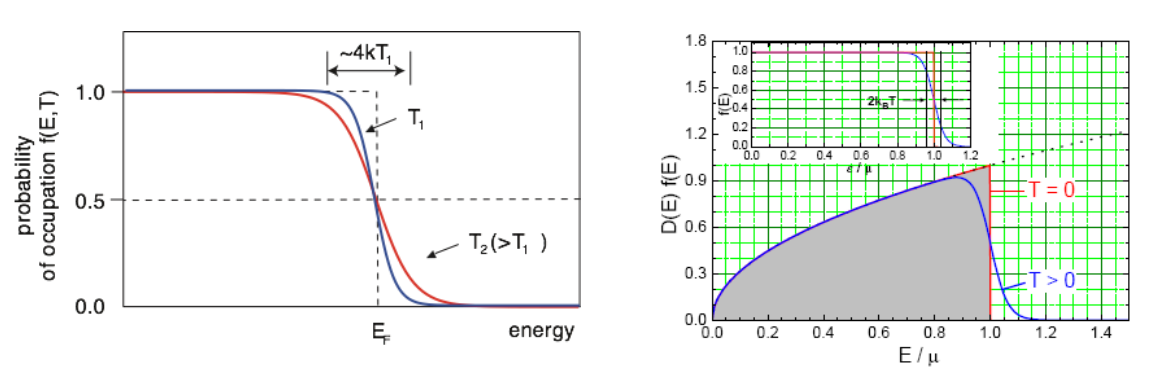
\includegraphics[width=\textwidth]{resources/24-03-2015/D(E)f(E).png}
    \caption{Fermifunktion und Zustandsdichte der Energie.}
    \label{fig:q58}
\end{figure}

\question{Was besagt das Bloch-Theorem bzw. die Bloch-Funktion?}
\label{q:59}

Bei einem periodischen Potential (z.B. der Überlagerung der Coulomb-Potentiale in einem Kristallgitter) können die Lösungen der Schrödinger Gleichung als Linearkombinationen von Basisfunktionen der Form

\[ \Psi_k(\vb{r}) = u_k(\vb{r}) e^{i\vb{k}\vb{r}}\]

mit \( u_k(\vb{r}) = u_k(\vb{r} + \vb{R}) \), d.h. mit einer Basis aus einer periodischen sogenannten Bloch-Funktion $u_k$ und einer Exponentialfunktion, dargestellt werden. Zeigen lässt sich dies, indem sowohl $\Psi$ als auch $U$ als komplexe Fourier-Reihe dargestellt werden. Die $u_k$ haben die Form

\[ u_k(\vb{R}) = \displaystyle \sum_{\vb{G}} c_{\vb{k}-\vb{G}}  e^{-i \vb{G} \vb{r}} \]

Die Fourier-Koeffizienten $c_{\vb{k}-\vb{G}}$ können aus folgendem Gleichungssystem berechnet werden, das auch als Hauptgleichung bezeichnet wird:

\[ \left( \frac{\hbar^2 k^2}{2m} - E \right) c_k + \displaystyle \sum_G U_G c_{k-G} = 0 \]

Dabei sind die $U_G$ die Koeffizienten der Fourier-Darstellung des Potenzials. Das Bloch-Theorem ist nützlich zur Berechnung der elektronischen Bandstruktur $E_n(k)$ eines Kristalls. 

\question{Welche Arten von Dia- und Paramagnetismus kennen Sie?}
\label{q:60}

Siehe \aqref{32}.

\newpage
\section{28. November 2018}
%! Hier gibts schon ein bisschen was hier: https://docs.google.com/document/d/1VvuRhqSy6umcpChijdMtuYw5qB0H7iJZGPXQbSMj6zA/edit
\question{Skizzieren Sie die wesentlichen Elemente der Born-Oppenheimer Näherung.}
\label{q:61}

Siehe \aqref{21}.


\question{Diskutieren Sie die sp-, sp2-, sp3-Hybridisierung in mehratomigen Molekülen.}
\label{q:62}

Hybridisierung bedeutet eine Mischung aus s- und p- Orbitalen,
hervorgerufen durch die Verformung der Elektronenhülle auf Grund
der Wechselwirkung zwischen den an der Bindung beteiligten Atomen.
Dabei gibt es die sp-, die sp2- und die sp3-Hybridisierung:

\begin{itemize}
    \item Eine sp-Hybridisierung führt zu zwei entgegengerichteten Bindungen und damit
          zu einem linearen Molekül, wenn keine anderen Bindungen vorhanden sind. Hier hybridisieren das 2s und ein 2p Orbital zu zwei sp-Orbitalen.
         
          \begin{figure}[H]
            \begin{minipage}[b]{0.5\linewidth} 
               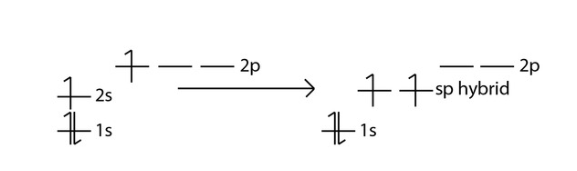
\includegraphics[width=0.8\linewidth]{resources/28-11-2018/sp11.PNG}
               \caption{sp-Hybridisierung, wobei die Energie sinkt}
            \end{minipage}
            \hspace{0.01\linewidth}
            \begin{minipage}[b]{0.5\linewidth} 
               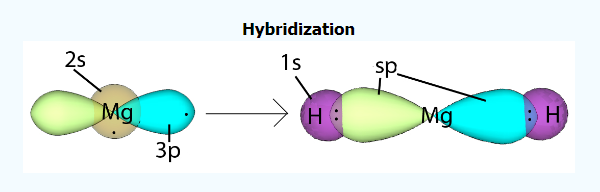
\includegraphics[width=0.8\linewidth]{resources/28-11-2018/sp12.PNG}
               \caption{sp-Hybridisierung am Beispiel von Magnesium }
            \end{minipage}
         \end{figure}

    \item Die sp2-Hybridisierung führt zu drei gerichteten Bindungen, die in einer
          Ebene liegen. Hier bilden sich aus den 2s und zwei 2p-Orbitalen, drei sp-Orbitale.

          \begin{figure}[H]
            \begin{minipage}[b]{0.5\linewidth} 
               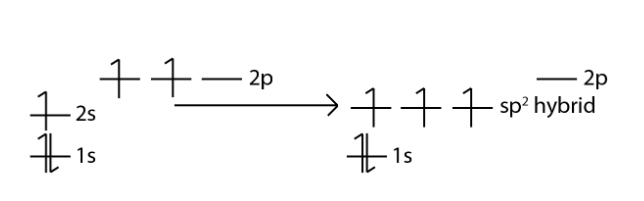
\includegraphics[width=0.8\linewidth]{resources/28-11-2018/sp21.PNG}
               \caption{sp2-Hybridisierung, wobei die Energie sinkt}
            \end{minipage}
            \hspace{0.01\linewidth}
            \begin{minipage}[b]{0.5\linewidth} 
               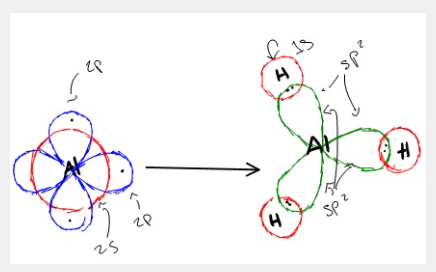
\includegraphics[width=0.8\linewidth]{resources/28-11-2018/sp22.PNG}
               \caption{sp2-Hybridisierung am Beispiel von Aluminiumhydroxid}
            \end{minipage}
         \end{figure}

    \item Für die sp3-Hybridisierung ergeben sich Atomorbitale mit Maxima, die in die vier Ecken eines Tetraeders zeigen.
          Hier bilden sich aus den 2s und drei 2p-Orbitalen, vier sp3-Orbitale.

          \begin{figure}[H]
            \begin{minipage}[b]{0.5\linewidth} 
               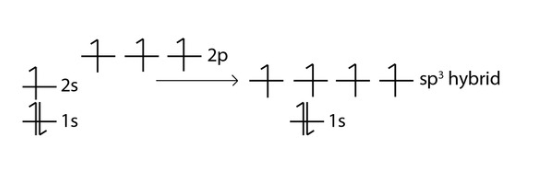
\includegraphics[width=0.8\linewidth]{resources/28-11-2018/sp31.PNG}
               \caption{sp3-Hybridisierung, wobei die Energie sinkt}
            \end{minipage}
            \hspace{0.01\linewidth}
            \begin{minipage}[b]{0.5\linewidth} 
               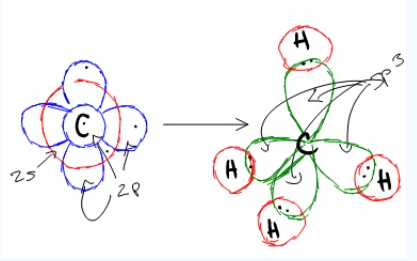
\includegraphics[width=0.8\linewidth]{resources/28-11-2018/sp32.PNG}
               \caption{sp3-Hybridisierung am Beispiel von Methan}
            \end{minipage}
         \end{figure}

\end{itemize}

\question{Diskutieren Sie die Laue'sche Beugungsbedingung anhand der Ewald-Konstruktion im Rahmen der Bragg'schen Interpretation.}
\label{q:63}

\question{Wodurch unterscheiden sich ein fcc-Gitter von einer hcp-Struktur?}
\label{q:64}

Siehe \aqref{46}.

\question{Diskutieren Sie die Gitterenergie der Ionenkristalle.}
\label{q:65}

\question{Vergleichen Sie die Einstein- und Debye-Modelle der spezifischen Wärme. Welche Annahmen sind in beiden Modellen zu einfach?}
\label{q:66}

\question{Diskutieren Sie das Auftreten einer Energiebandlücke mit Hilfe des Modells der fast freien Elektronen.}
\label{q:67}

siehe \aqref{5}

\question{Wodurch unterscheidet sich die Dispersionsrelation der Phononen eines primitiven kubischen Gitters von jenem eines CsCl-Gitters.}
\label{q:68}

\question{Erklären Sie die chemische Bindung von \ch{O2} ($Z=8$).}
\label{q:69}

\[\ch{O2} : (1\sigma_g)^2 ~ (1\sigma_u^*)^2 ~ (2\sigma_g)^2 ~ (2\sigma_u^*)^2 ~ (3\sigma_g)^2 ~ (1\pi_g)^4 ~ (1\pi_u^*)^2\]

Da beide Sauerstoffatome je zwei freie Valenzelektronen haben, kommt es zu einer Doppelbindung.

\setcapindent{0pt}
\begin{figure}[H]
   \centering
   \begin{minipage}[t]{0.475\linewidth}
      \centering
      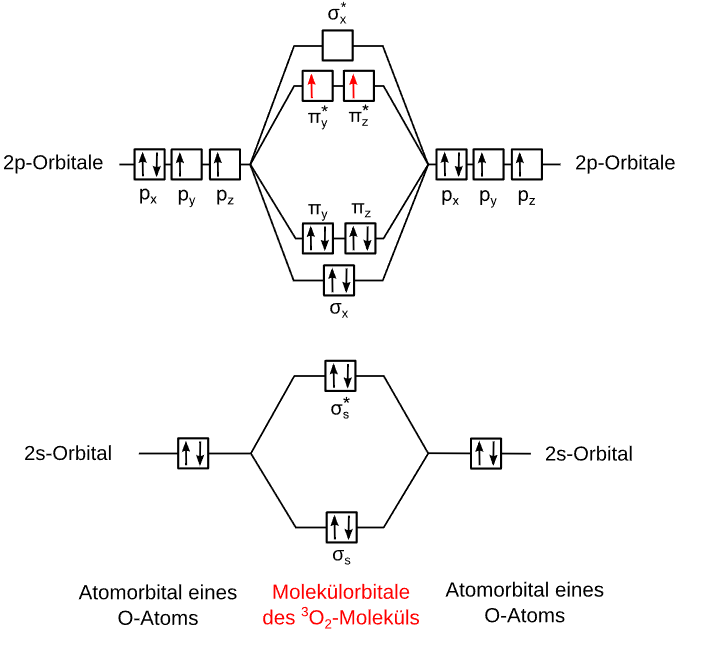
\includegraphics[width=\linewidth]{resources/28-11-2018/O2.PNG}
      \caption{Elektronenkonfiguration von \ch{O2}}
      \label{fig:Elektronenkonfiguration_O2}
   \end{minipage}%
   \hspace*{\fill}
   \begin{minipage}[t]{0.475\linewidth}
      \centering
      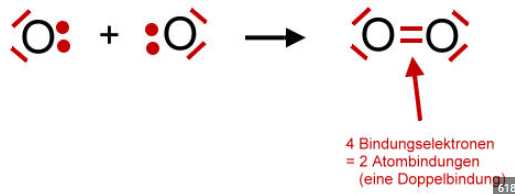
\includegraphics[width=\linewidth]{resources/28-11-2018/o2_bindung.PNG}
      \caption{Chemische Bindung zweier Sauerstoffatome}
      \label{fig:chemische_Bindung_O2}
   \end{minipage}
\end{figure}
\setcaphanging

\newpage
\section{31. Oktober 2013}

\question{Bindungszustände / Elektronenkonfiguration in \ch{N2} diskutieren.}
\label{q:70}

Siehe \aqref{52}.

\question{Skizzieren Sie die wesentlichen Elemente der Born-Oppenheimer Näherung.}
\label{q:71}

Siehe \aqref{21}.

\question{Erklärung von Hybridisierung anhand sp, sp2 und sp3.}
\label{q:72}

\question{Lennard-Jones Potential und Van der Waals Bindung.}
\label{q:73}

Van der Waals Kräfte sind die relativ schwachen nicht weitreichende Wechselwirkungen zwischen Atomen oder Molekülen. Sie können ideale Gas Atome zusammenhalten, obwohl diese aufgrund ihrer neutralität keine Coulomb Anziehung zwischen sich haben.
Normalerweise ist das Dipolmoment eines solchen Atoms 0, jedoch kann durch Schwankungen der Ladung um ihre Durchschnittliche Position kurzzeitig eines entstehen. 
Das Nachbaratom reagiert auf dieses und es kommt zu einer anziehenden Kraft zwischen ihnen. Der Durchschnitt der Kräfte zwischen den Atomen ist die Van-der-Waals-Kraft. Diese Bindungen sind sehr schwach und die Bindungsenergie beträgt nur wenige meV.
Das Van-der-Waals Bindungspotential ist oft durch das Lennard-Jones-Potential angenähert. Dieses beschreibt in der Atom- und Molekülphysik die Bindungsenergie. Es nähert die Wechselwirkung zwischen ungeladenen, nicht chemisch aneinander gebundenen Atomen an.

\begin{align}
    U(R) = 4\epsilon[(\frac{\sigma}{R})^{12} - (\frac{\sigma}{R})^6]
\end{align}

Dabei entspricht $\epsilon$ der Tiefe der Potentialmulde, $\sigma$ dem Teilchenabstand an der Nullstelle und $R$ dem variierendem Abstand der Teilchen.\\

\begin{figure}[H]
    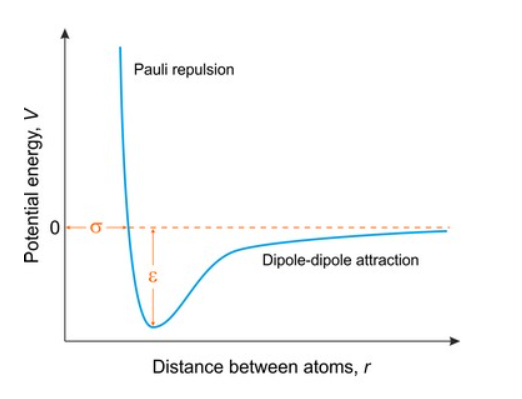
\includegraphics[width=0.8\linewidth]{resources/31-10-2013/lennard.PNG}
    \caption{Beispielhafter Plot des Lennard-Jones-Potentials}
\end{figure}

\question{Diskutieren Sie die Laue'sche Beugungsbedingung.\
\qquad \qquad a) Anhand der Ewald-Konstruktion.\
\qquad \qquad b) Im Rahmen der Bragg'schen Interpretation.}
\label{q:74}

\question{Skizzieren Sie die 1. Brillouin-Zone eines ebenen hexagonalen Gitters.}
\label{q:75}

\begin{figure}[H]
    \centering
    \begin{samepage}
        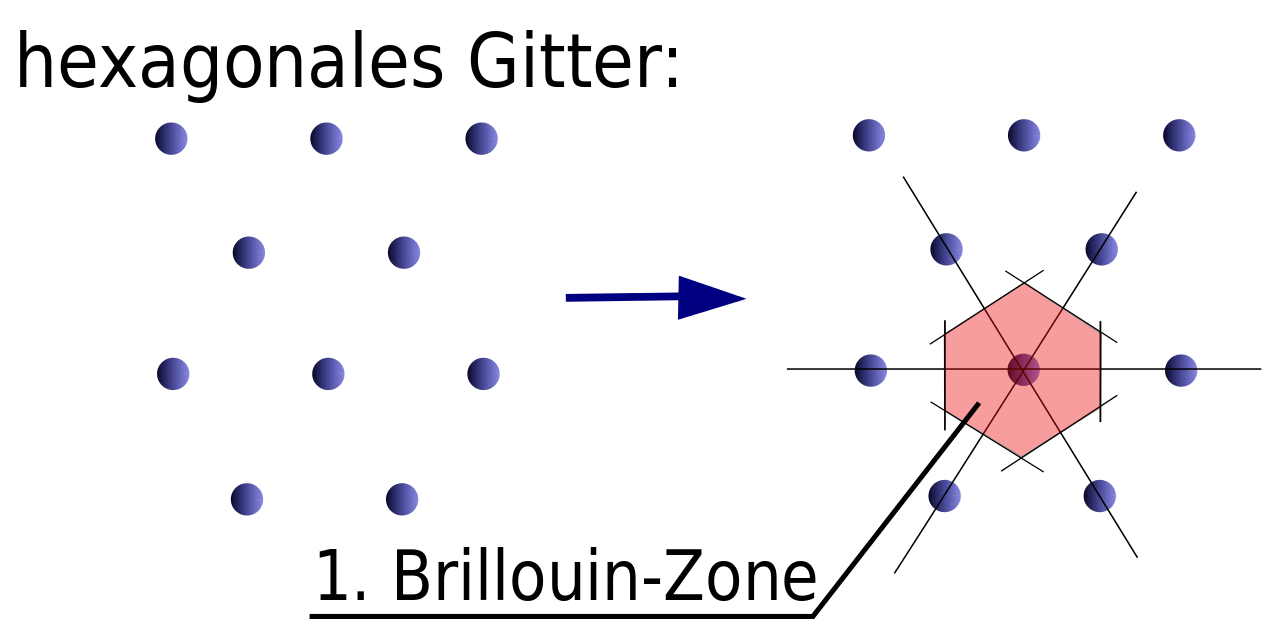
\includegraphics[width=0.6\linewidth]{resources/31-10-2013/BZ1_hexagonal.png}
        \caption{1. Brillouin-Zone eines hexagonalen Gitters}
    \end{samepage}
\end{figure}

\question{Gitterenergie in einem Ionenkristall.}
\label{q:76}

siehe \aqref{65}

\question{Röntgenbeugung mit der Drehkristallmethode.}
\label{q:77}

\question{Vergleichen Sie das Einstein- und Debye-Modell der spezifischen Wärme. Welche Annahme ist in BEIDEN Modellen zu einfach?}
\label{q:78}

siehe \aqref{57}

\newpage
\section{Juli 2017}

\question{Zeichne das Potential eines homöopolaren Moleküls. Beschreiben Sie es qualitativ.}
\label{q:79}

siehe \aqref{11}

\question{Was bewirkt die Austauschenergie beim H2 Molekül? Wann ist sie groß/klein? Wieso ist sie für die chemische Bindung wichtig?}
\label{q:80}

Siehe \aqref{1}.

\question{Was kann man aus dem Rotations-Schwingungsspektrum für molekulare Größen bestimmen?}
\label{q:81}

Siehe \aqref{2}.

\question{Diskutieren Sie elektrische Rotations-Schwingungsübergänge und die Entstehung von Schwingungsbanden.}
\label{q:82}

Siehe \aqref{3}.

\question{Wie kann experimentell die Dispersionsrelationskurve von Phononen ermittelt werden?}
\label{q:83}

siehe \aqref{6}.

\question{Diskutieren Sie die Wärmekapazität sowohl in der klassischen als auch in der quantenmechanischen Betrachtung.}
\label{q:84}

siehe \aqref{7}.

\question{Was für ein Zusammenhang besteht zwischen der Gitterebene und einem Vektor im reziproken Raum?}
\label{q:85}

Siehe \aqref{4}.

\question{Erklären Sie das Auftreten von Energiebandlücken mit Hilfe des Models der fast freien Elektronen.}
\label{q:86}

siehe \aqref{5}

\question{Beschreiben Sie das Bloch-Theorem eines Elektrons im harmonischen Potential.}
\label{q:87}

siehe \aqref{8}.

\question{Diskutieren Sie die Zustandsdichte in Schwingungsspektren von Festkörpern.}
\label{q:88}
\end{document}